\documentclass[12pt]{article}

\usepackage{amssymb,amsmath}
\usepackage[margin=1.0in]{geometry}
\usepackage{fancyhdr} % required for custom header
\usepackage{graphicx}
\usepackage{listings}
\usepackage{courier}
\usepackage[usenames,dvipsnames]{color}
\usepackage[maxfloats=40]{morefloats}
\usepackage{caption}
\usepackage{subcaption}
\usepackage{natbib}


%set up the header
\pagestyle{fancy}
\lhead{Trever Hines}
\chead{El Mayor Postseismic}
\rhead{\today}

\setlength{\headheight}{15pt}
\renewcommand\headrulewidth{1.0pt} % Size of the header rule

%% Title
%%------------------------------------------------------------------------------
\title{	
El Mayor Postseismic
\author{Trever Hines}
\rule{\headwidth}{1.0pt}
}

 
 
\begin{document}
\maketitle
\section*{Abstract}
we propose a anelastic phase of deformation in the mantle distinct from phases associated with attenuation

\section{Introduction}

Previous studies which have modeled postseismic deformation following the El Mayor-Cucapah earthquake include \citet{Pollitz2012}, \citet{Gonzalez-ortega2014}, \citet{Spinler2015}, and \citet{Rollins2015}. \citet{Gonzalez-ortega2014} was able to describe five months of near field ($\lesssim 50$ km from the epicenter) postseismic defomation observed by InSAR and campaign GPS with afterslip and fault contraction on the coseismically ruptured fault. \citet{Gonzalez-ortega2014} also noted that their preferred model underestimated the GPS displacements for stations $\gtrsim 25$ km from the rupture and suggested that it could be the result of unmodeled viscoelastic relaxation.  Using continuous GPS stations within 200 km of the El Mayor-Cucapah epicent, which consists mostly of stations north of the US-Mexico border, \citet{Rollins2015} found that three years of postseismic deformation can be adequately explained by afterslip in an elastic lithosphere, albeit with an implausibly large amount of afterslip inferred on the least constrained southern most fault segment which may be acting as a proxy for distributed relaxation in the lower crust or upper mantle. In this paper, we reiterate this finding by \citet{Rollins2015} and note that a purely elastic dislocation model is incapable of describing deformation observed at GPS stations greater than ~200 km from the El Mayor-Cucapah epicenter.  

Given the inability to describe both near and far field deformation with fault slip in an elastic lithosphere, \citet{Pollitz2012}, \citet{Rollins2015} and \citet{Spinler2015} have explored viscoelastic relaxation in the lower crust and upper mantle as a potential deformation mechanism. The lithospheric rheology is largely unknown and so modeling postseismic deformation with viscoelastic relaxation requires one to assume a rheologic model and find the best fitting model parameters, which is generally a computationally expensive nonlinear inverse problem. Consequently, a simplified structure for the lithosphere must be made to minimize the number of rheologic parameters that need to be estimated.  For example, it is commonly assumed that the lithosphere consists of only three homogeneously Maxwell viscoelastic layers, which may be an inadequate representation of the lithosphere \citep[e.g.][]{Hines2013,Riva2009}. Additionally, it is necessary to make simplifying assumptions about the nature of afterslip. For example, one can assume a frictional model for afterslip and parameterize afterslip in terms its the unknown rheologic properties \citep[e.g.][]{Johnson2009,Johnson2004}. Additionally, one can assume that afterslip only dominates the first year of deformation \citep[e.g.][]{Pollitz2012,Spinler2015} and that viscoelastic relaxation is the dominant mechanism in later years. However, numerous observations of interseismic fault creep has been recognized in this and similar tectonic settings and it has been speculated that such creep can be initiated as a postseismic process \citep{Cakir2012,Cetin2014}.  We therefore do not make to implicit assumption that afterslip terminates after a given amount of time.  Indeed, the preferred viscoelastic model from \citet{Pollitz2012} underestimates near field velocities, which could be indicative of unmodeled continued afterslip.

All of the aforementioned studies model displacements observered at stations within 200 km of the El Mayor-Cucapah epicenter, while postseismic deformation in this region following previous earthquakes of similar magnitude has been observed at distances extended out to about 300 km \citep{Freed2007a}. In the present study we examine stations within 400 km of the El Mayor-Cucapah epicenter, which turns out to be crucial for discerning the postseismic deformation mechanism.

Clearly, both afterslip and viscoelastic relaxation are involved in postseismic deformation neglecting to model one of these deformation mechanisms could result in a biased estimate of the other.  In this paper we use the inverse method described in \citet{Hines2015} to estimate the afterslip an effective viscosity necessary to describe the transience postseismic deformation over the first ten months after the El Mayor-Cucapah earthquake. We then form a suite of models which have various lithospheric rheologies but viscosities that are consistent with the effective viscosity estimated from the early postseismic deformation. Of the suite of models tested, we find that five years of postseismic deformation can be explained by a combination of sustained afterslip on the coseismicly ruptured fault and a Zener rheology upper mantle with viscosity that decays from $\sim5\times10^{18}$ to $\sim1\times10^{18}$ Pa s. 


\section{Data Processing}\label{sec:Data}

We use continuous GPS position time series provided by University Navstar Consortium (UNAVCO) stations within a 400 km radius about the El Mayor-Cucapah epicenter. Our analysis is on the coseismic and postseismic displacement resulting from the El Mayor-Cucapah earthquake, which we collectively describe as $u(t)$. We consider GPS position time series, $u_\mathrm{obs}(t)$, to be the superposition of $u(t)$, secular tectonic deformation, annual and semi-annual oscillations, and coseismic offsets from significant earthquakes over the time span of this study.  The June 14, 2010 Mw5.8 Ocotillo earthquake and the August 26, 2012 Brawley swarm, which consisted of a Mw5.5 and Mw5.3 event (figure \ref{fig:ContextMap}), are the only earthquakes after the El Mayor-Cucapah earthquake that produced noticeable offsets recorded by GPS. Although the Ocotillo earthquake had its own series of aftershocks \citep{Hauksson2011}, neither earthquake produced detectable postseismic deformation of its own. We thus model $u_\mathrm{obs}(t)$ as 
\begin{equation}
  u_\mathrm{obs}(t) = u_\mathrm{pred}(t) + \epsilon
\end{equation}
where
\begin{equation}\label{TimeSeriesModel}
  \begin{split}  
    u_\mathrm{pred}(t) = &u(t)H(t-t_\mathrm{emc}) + c_0 + c_1t + \\
                         &c_2\sin(2\pi t) + c_3\cos(2\pi t) + c_4\sin(4\pi t) + c_5\cos(4\pi t) + \\
                         &c_6H(t-t_\mathrm{oc}) + c_7H(t-t_\mathrm{bs}).
  \end{split}
\end{equation}
In the above equations, $t_\mathrm{emc}$, $t_\mathrm{oc}$ and $t_\mathrm{bs}$ are the times of the El Mayor-Cucapah earthuqake, Ocotillo earthquake, and the Brawley swarm respectively, $H(t)$ is the Heaviside function, $c_0$ through $c_7$ are unknown coefficients, and $\epsilon$ is the observation noise. We only estimate jumps associated with the Ocotillo earthquake and Brawley swarm for stations within 40 km of their epicenters. 

Stations which recorded signals that clearly cannot be described by the aforementioned processes are not included in our analysis. This includes stations in the Los Angeles basin, which record deformation that is largely anthropogenic. In order to ensure an accurate estimation of the secular deformation, we only use stations that were installed at least six months prior to El Mayor-Cucapah earthquake. Several GPS stations were installed after the El Mayor-Cucapah earthquake to improve the spatial resolution of postseismic deformation \citep{Spinler2015} and it is possible to subtract secular velocities derived from elastic block models \citep[e.g.][]{Meade2005} from velocities recorded at the newly installed stations to get an estimate of postseismic velocities. However, we use coseismic and postseismic displacements, rather than velocities, in our inverse method described in section \ref{sec:Model} because estimating velocities from an already noisy displacement time series can introduce significant aleatoric and epistemic uncertanties depending on exactly how the estimation is done. This modeling choice prevents us from using the newly installed stations in Baja California in our analysis.   

The October 16, 1999 Hector Mine earthquake, which occurred within our study region about 270 km north of the El Mayor-Cucapah epicenter, has produce transient postseismic deformation which we do not wish to model either mechanically or through empirical line fitting. We thus restrict our analysis to deformation observed six years after the Hector Mine earthquake, past which point postseismic velocities at sites proximal to the Hector Mine epicenter are approximately constant \citep{Savage2009}.  When appraising our model fit in section \ref{sec:Model}, we see some systematic residuals in the vicinity of the Hector Mine, which may be the result of errors in this approximation.   

Studies of postseismic deformation typically assume a parametric form for $u(t)$, such as one with a logarithmic or exponential time dependence \citep[e.g.][]{Savage2005a}.  However, by assuming a logarithmic or exponential form of $u(t)$ we run the risk of over fitting the GPS time series and inferring a nonexistent postseismic signal. We therefore do not assume any parametric form for $u(t)$ and rather treat it as integrated Brownian motion, so that 
\begin{equation}
    \dot{u}(t) = \sigma^2\int_0^t w(s) ds.
\end{equation}    
where $w(t)$ is white noise and the variance of $\dot{u}(t)$ increases linearly with time by a factor of $\sigma^2$. We use a Kalman filtering approach to estimate $u(t)$ and the unknown parameters in eq. \ref{TimeSeriesModel}.  In the context of Kalman filtering, our time varying state vector is
\begin{equation}
    \mathbf{X}(t) = [u(t),\dot u(t), c_0, ..., c_7]
\end{equation}
and eq. \ref{TimeSeriesModel} is the observation function which maps the state vector to the GPS observations. We initiate the Kalman filter by assuming a prior estimate of $\mathbf{X}(t)$ at the first time epoch, denoted $\mathbf{X}_{1|0}$, which has a sufficiently large covariance, denoted $\mathbf{\Sigma}_{1|0}$, to effectively make our prior uninformed.  For each time epoch, $t_i$, Bayesian linear regression is used to incorporate GPS derived estimates of displacement with our prior estimate of the state, $\mathbf{X}_{i|i-1}$, to form a posterior estimate of the state, $\mathbf{X}_{i|i}$, which has covariance $\mathbf{\Sigma}_{i|i}$.  

We then use the posterior estimate of the state at time $t_i$ to form a prior estimate of the state at time $t_{i+1}$ through the transition function
\begin{equation}\label{predict}
  \mathbf{X}_{i+1|i} = \mathbf{F}_{i+1}\mathbf{X}_{i|i} + \mathbf{\delta}_{i+1} 
\end{equation}
where 
\begin{equation}
  \mathbf{F}_{i+1} = 
  \left[
  \begin{array}{ccc}
    1           & (t_{i+1} - t_i) & \mathbf{0}\\
    0           & 1              & \mathbf{0}\\
    \mathbf{0}  & \mathbf{0}     & \mathbf{I}
  \end{array}
  \right]
\end{equation}
and $\mathbf{\delta}_{i+1}$ is the process noise, which has zero mean and covariance described by
\begin{equation}
  \mathbf{Q}_{i+1} = 
  \sigma^2 \left[
  \begin{array}{ccc}
  \frac{(t_{i+1} - t_i)^3}{3} & \frac{(t_{i+1} - t_{i})^2}{2} & \mathbf{0}\\
  \frac{(t_{i+1} - t_i)^2}{2} & (t_{i+1} - t_{i}) & \mathbf{0}\\ 
  \mathbf{0} & \mathbf{0} & \mathbf{0}
  \end{array}
  \right].
\end{equation}

The covariance of the new prior state, $\mathbf{X}_{i+1|i}$, is then described by
\begin{equation}
  \mathbf{\Sigma}_{i+1|i} = \mathbf{F}_{i+1}\mathbf{\Sigma}_{i|i}\mathbf{F}^T_{i+1} + \mathbf{Q}_{i+1}.
\end{equation}

This process is repeated for each of the $N$ time epochs at which point we use Rauch-Tung-Striebel smoothing \citep{Rauch1965} to find $\mathbf{X}_{i|N}$, which is an estimate of the state at time $t_i$ that incorporates GPS observation for all $N$ time epochs.  Our final estimates of $u(t)$ are used in subsequent analysis, while the remaining components of the state vector are considered nuisance parameters. In the interests of computational tractability, we down sample our smoothed time series from daily solutions down to weekly solutions.

The smoothness of $u(t)$ is controlled by the chosen value of $\sigma^2$, which describes how rapidly we expect the postseismic signal to vary over time.  Setting $\sigma^2$ equal to zero will effectively result in modeling $u(t)$ as a straight line which is insufficient to describe the expected transient behaviour in postseismic deformation. The other end member, where $\sigma^2$ is infinitely large, will result in $u_\mathrm{pred}(t)$ fitting what is obviously noise in the data. While one can use a maximum likelihood based approach to picking $\sigma^2$ \citep[e.g.][]{Segall1997}, we rather take a subjective approach and choose a value for $\sigma^2$ that is just large enough to faithfully describe the postseismic deformation at the most near field station in our study, P496, which exhibits the most pronounced rapid changes in velocity. This ensures that $\sigma^2$ will be sufficiently large so that our estimate of $u(t)$ does not smooth out potentially valuable postseismic signal at the remaining stations. We find that when using $\sigma^2 = 0.05 \mathrm{m}^2 / \mathrm{yr}^3$, we are able to adequately describe all but the first week of postseismic deformation at station P496, which gets incorporated into our estimate of coseismic displacements (figure \ref{fig:P496Fit}). We assume that the first week of deformation is overwhelmingly the result of afterslip and any unmodeled afterslip over the first week following the El Mayor-Cucapah earthquake will be added into our estimates of coseismic slip in section \ref{sec:Model}.  Figure \ref{fig:P496PS} shows the estimate of coseismic and postseismic deformation, $u(t)$, for station P496 along with the estimated uncertainties. \cite{Freed2007a} noted that postseismic deformation can be observed at distances greater than 200 km from the Hector Mine earthquake and indeed, after processing the time series for stations up to 400 km from the El Mayor-Cucapah epicenter, we see clear postseismic transient deformation (\ref{fig:P619Fit} and \ref{fig:P619PS}).      

It is important to note that the shown uncertainties in $u(t)$ do not account for the non-negligible epistemic uncertainty in eq. \ref{TimeSeriesModel}.  For example, we assume a constant secular rate of deformation, while viscoelastic mechanical models of the earthquake cycle predict that the accumulation of tectonic deformation is nonlinear over time \citep{Thatcher1983}. Based on inspection, the rate of secular deformation does appear constant for all stations except for perhaps the stations closest to the Hector Mine epicenter, as noted aboved.  Also, our model for seasonal deformation in eq. \ref{TimeSeriesModel} assumes a constant amplitude over time, which means that years of particularly heavy or light rainfall cannot be adequately described.  This deficiency in our seasonal model causes our estimate of $u(t)$ to describe some of the unmodeled oscillations (e.g. figure \ref{fig:P619PS}).          

We show the near and far field postseismic deformation accumulated over the intervals  0-0.8 years, 0.8-3.0 years, and 3.0-5.0 years, as well as coseismic displacements in figures \ref{fig:NearField1} through \ref{fig:FarField4}.  In the far field, we can see clear south trending displacement for the first 3.0 years following the earthquake at stations as far as 400 km from of the El Mayor Cucapah epicenter.  These displacements are most pronounced along the direction of the El Mayor-Cucapah P and T axis, as would be expected for postseismic deformation. After 3.0 years, The southward trending far field postseismic deformation is barely perceptible.  The vertical deformation in the far field is difficult to attribute to postseismic processes.  Most far field stations display an initial subsidence for the first year after the El Mayor-Cucapah earthquake followed by continued uplift.  This trend in vertical deformation can be observed in all three of the quadrants where postseismic data is available, which means that the vertical deformation does not exhibit an anti-symetric quadrant pattern, as would be expected for postseismic processes.  Although we use vertical deformation in our analysis in section \ref{sec:Model},  we do not put an emphasis on trying to describe the vertical deformation as it likely has non-tectonic origins.        

The near field postseismic deformation is notably sustained when compared to the far field deformation.  Namely, the station in this study which is closest to the El Mayor-Cucapah epicenter, P496, is moving at a steady rate of ~1.4 cm/yr to the south five years after the El Mayor-Cucapah earthquake.  Vertical postseismic deformation in the near field does display a quadrant pattern which is consistent with the coseismic vertical deformation, suggesting that it is indeed resulting from tectonic processes.  However, the vertical postseismic deformation signal is only apparent in the early postseismic period (figure \ref{fig:NearField2}).  As with the far field deformation, there is a general trend of uplift in the near field one year after the earthquake which we do not consider to be related to postseismic processes.  

\section{Postseismic Modeling}\label{sec:Model}

In this paper, we seek to find the mechanisms driving five years of postseismic deformation following the El Mayor-Cucapah earthquake. We consider afterslip and viscoelastic relaxation in the lithosphere and/or asthenosphere as candidate mechanisms.  Poroelastic rebound has also been used to model postseismic deformation \citep[e.g.][]{Jonsson2003}; however, \cite{Gonzalez-ortega2014} suggest that any contribution to postseismic deformation from poroelastic rebound would be negligible.  Additionally, we are considering stations which are sufficiently far away from the main rupture that poroelastic rebound should be insignificant.  

We estimate coseismic and time dependent postseismic fault slip, both of which are assumed to occur on the fault geometry estimated by \citet{Wei2011} with some modifications.  Field studies \citep{Fletcher2014} and LIDAR observations \citep{Oskin2012} have revealed a significantly more complicated fault geometry than what was inferred by \citet{Wei2011}, especially within the Sierra Cucapah.  However, we find the relatively simple coseismic fault geometry from \cite{Wei2011} to be sufficient because most of the stations used in this study are sufficiently far from the El Mayor-Cucapah rupture zone that they are insensitive to the details in the fault geometry found by \cite{Fletcher2014} and \cite{Oskin2012}.  The fault geometry used in this study (figure \ref{fig:ContextMap}) consists of the two main fault segments inferred by \cite{Wei2011}, where the northern segment runs through the Sierra Cucapah up to the US-Mexico border and the southern segment is the Indiviso fault which extends down to the Gulf of California.  Additionally, We extend the northern segment by 40 km to the northwest which is motivated by the clustering of aftershocks on the northern tip of the coseismic rupture zone \citep{Hauksson2011,Kroll2013}.  This extended fault segment was also found to be necessary by \cite{Rollins2015} and \cite{Pollitz2012} for describing postseismic deformation.     

We consider a variety of rheologic models for the lithosphere and asthenosphere in this study.  The simplest rheologic model is to consider the lithospere and asthenosphere to be effectively elastic and isotropic.  In such case, the rheologic parameters, consisting of the Lame parameters, $\lambda$ and $\mu$, and density, $\rho$, are reasonably well known. The only unknowns are then the distribution of fault slip, which can be easily estimated due to the linearity of the forward problem.  \cite{Rollins2015} found that postseismic deformation following the El Mayor-Cucapah earthquake can be well explained with afterslip on the coseismicly ruptured fault, which has been extended down to the lithosphere-asthenosphere boundary inferred by \cite{Lekic2011}, and they did not require any viscoelastic relaxation to describe the observations.  They did however, find that an unrealistically large amount of afterslip is required on the Indiviso fault, equivalent to a Mw7.2 earthquake.  Since most of the GPS data is located north of the rupture zone, slip on the Indiviso fault segment is not well constrained and it could be acting as a proxy for distributed relaxation in the lower crust or upper mantle.  It is well understood that afterslip at sufficiently great depths can explain postseismic deformation resulting from viscoelastic relaxation \cite{Savage1990}, at least in 2D earthquake models.  In the interest of eliminating null space in our inverse problem,  we assume that afterslip occurs only at seismogenic depths ($<15$ km), and we allow for viscoelastic relaxation in the lower crust (15-30 km) and the upper mantle.  We choose such shallow constraints on afterslip because rate-state friction based models would suggest afterslip to occur at shallow depths to accommodate a coseismic slip deficit \cite{Marone1991}, which is indeed inferred in the coseismic models by \cite{Wei2011a} and (Fialko 2010).  Additionally, as noted by \cite{Rollins2015} the postseismic uplift just north of the rupture zone can be well described with slip at seismogenic depths, while afterslip which is constrained to depths below 15 km predicts subsidence in that region.  

Another reason for constraining slip to be shallower than 15 km depth is because we seek to estimate a lower crustal viscosity and the inverse problem becomes particularly ill-posed when trying to simultaneously estimate afterslip and a lithospheric viscosity at the same depths. 
This ill-posedness is illustrated in figure (\ref{fig:LowerCrust}), which shows the displacement resulting from a meter of slip on a fault extending from 15 to 30 km depth as well as the initial velocity resulting from viscoelastic relaxation in the lower crust, which is given a viscosity of $10^{18}$ Pa s.  The horizontal displacement from fault slip is in the opposite direction as the displacements resulting from subsequent viscoelastic relaxation.  This means that displacement resulting from afterslip at lower crustal depths can be cancelled out, at least partially, by a low viscosity lower crust.  We eliminate this null space by allowing only one mechanism in the lower crust, which we choose to be viscoelastic relaxation.  Aside from the issue of non-uniqueness, it is also nonsensical to allow for both brittle and ductile deformation mechanisms at the same depth. 

A schematic representation of the viscoelastic rheologic models considered in this study for the lower crust and upper mantle are shown in figure \ref{fig:Rheology}.  We consider Maxwell viscoelasticity, where the steady state viscosity $\eta_M$ is unknown; Zener viscoelasticty, where the transient viscosity $\eta_K$ and transient shear modulus $\mu_K$ are unknown; and Burgers viscoelasticity, where $\eta_M$, $\eta_K$, and $\mu_K$, are all largely unknown. We further discuss these rheologic models and their use in geophysical studies in the discussion. 

\subsection*{constraint on effective viscosity}\label{InitialInversion}
For any linear viscoelastic rheology of the lithosphere and asthenosphere, postseismic displacement resulting from time dependent fault slip, $s(\xi,t)$, on a fault $F$ can be described as  
\begin{equation}\label{GeneralForward}
  u(x,t) = \int_F s(\xi,t)g(x,\xi)d\xi + 
           \int_0^t\int_F s(\xi,\tau) f(t-\tau,x,\xi) d\xi d\tau
\end{equation}
where $g(x,\xi)$ describes the instantaneous elastic displacements at $x$ resulting from a unit of slip at $\xi$, and $f(t,x,\xi)$ describes the time dependent velocity at $x$ resulting from viscoelastic relaxation of stresses induced by slip at $\xi$. $f$ is a function of the properties of the chosen rheologic model, which are generally not well known.  The parameters controlling the instantaneous elastic behaviour of the lithosphere and asthenosphere, $\mu$, $\lambda$, and density $\rho$, are relatively well known and we use the values listed in table (TBD), which are consistent with the properties used in the coseismic model by \cite{Wei2011} and the 1D SCEC background velocity model.  The remaining rheologic parameter, which we will assume to have a depth dependence, are estimated to optimize the predicted fit to observable postseismic displacement.

In order to greatly simplify the posed inverse problem, we use to method describe in \cite{Hines2015} to constrain the effective lithospheric viscosity structure for the early postseismic period.  The method relies upon the fact that immediately after an earthquake, stresses throughout the lithosphere and asthenosphere are controlled by the relatively well known instantaneous elastic properties.  This means that the rate of deformation in each parcel of the lithosphere will deform at a rate that is inversely proportional to its effective viscosity, $\eta_{\mathrm{eff}}=\frac{\sigma}{\dot{\epsilon}}|_{t=0}$, and independent of $\eta_{\mathrm{eff}}$ elsewhere. Then, as a consequence of linear elasticity, the initial rate of surface deformation resulting from viscoelastic relaxation is a linear combination of the surface deformation resulting from each parcel, scaled by the reciprocal of the parcel's viscosity. That is to say   
\begin{equation}\label{InitialRate}
  f(0,x,\xi) = \int_L \frac{h(x,\xi,\zeta)}{\eta_\mathrm{eff}(\zeta)} d\zeta, 
\end{equation}
where $h(x,\xi,\zeta)$ describes the initial rate of deformation resultion from viscoelastic relaxation at $\zeta$ induced by slip at $\xi$ and $L$ denotes the lithosphere and asthenosphere. Importantly, $h$ is independent of all rheologic properties other than those that control the instantaneous elastic behaviour, $\mu$, $\lambda$ and $\rho$. We can combine eq. \ref{InitialRate} with \ref{GeneralForward} to get a first order approximation for early postseismic deformation,
\begin{equation}\label{ApproxForward}
  u(x,t) \approx \int_F s(\xi,t)g(x,\xi)d\xi + 
           \int_0^t\int_F\int_L \frac{s(\tau,\xi)}{\eta_\mathrm{eff}(\zeta)} h(x,\xi,\zeta) d\zeta d\xi d\tau,
\end{equation}
which is valid for as long as the rate of deformation resulting from viscoelastic relaxation is approximately constant. Although eq. \ref{ApproxForward} may only be valid for a short portion of the postseismic period, its utility becomes apparent when noting that $g$ and $h$ are functions of the fault geometry and instantaneous elastic properties, which are fairly well known, and so $g$ and $h$ can be computed numerically as a preprocessing step and the forward problem, eq. \ref{ApproxForward}, can be rapidly evaluated for any realization of $s$ and $\eta_{\mathrm{eff}}$.  This is in contrast to evaluating the full forward problem, eq. \ref{GeneralForward}, numerically for each realization of $s$ and unkown rheologic properties which is far more computationally demanding. Figure \ref{fig:Rheology} shows how $\eta_\mathrm{eff}$ relates to the parameters for various linear viscoelastic rheologies.    

We perform an initial inversion of postseismic displacements using eq. \ref{ApproxForward} as our forward problem. As noted, we use the fault geometry from \citet{Wei2011}, except that each segment extends to 15 km depth and the north segment is extended 40 km northward.  Each fault segment is discretized into roughly 4 km by 4 km patches and we estimate a strike-slip and thrust component of slip for each patch. We estimate coseismic slip as well as the rate of afterslip over time intervals spanning 0.0-0.125 years, 0.125-0.25 years, 0.5-1.0 years, and at 1.0 year intervals for the remaining five years.  We impose that the coseismic slip and rates of afterslip are within 45$^\circ$ of right-lateral slip.  We estimate $\eta_{\mathrm{eff}}$ within six vertically stratified layers which have depths ranging from 15-30 km, 30-60 km, 60-90 km, 90-120 km, 120-150 km, and 150 km to the bottom of our numerical model domain, 800 km. Details of the inverse method are described in \citet{Hines2015}.  We note that a nonlinear Kalman filter based inverse method can be employed to estimate $s$ and $\eta_{\mathrm{eff}}$ in a manner akin to \citet{Segall1997} or \citet{McGuire2003}, where we do not have to explicitly impose a time dependent parameterization of $s$. Indeed we have thoroughly explored that possibility but we ultimately prefer the method described in \citet{Hines2015} because of its relative simplicity and because we believe the piecewise continuous respresentation of slip with respect to time to be sufficiently general.

The first step in our inverse method is to determine at which point the early postseismic approximation, eq. \ref{ApproxForward}, is no longer approriate, which we will denote as $t_{\mathrm{end}}$.  As noted, it is valid for approximately as long as the rate of deformation resulting from viscoelastic relaxation is approximately constant. We can almost certainly assume that deformation at the most far field stations which are $\sim400$ km away from the El Mayor-Cucapah epicenter is the result of viscoelastic relaxation. The approximation should then be valid for as long as a linear trend adequately approximates the far field deformation. Using this logic, it would appear that $t_{\mathrm{end}}$ is $\sim1$ year after the El Mayor-Cucapah earthquake.  Another way to determine $t_{\mathrm{end}}$ is to find the best fitting prediction of eq. \ref{ApproxForward} to observed deformation using increasing durations of the postseismic timeseries.  $t_\mathrm{end}$ should be the point when eq. \ref{ApproxForward} is not longer capable of describing the observed deformation without incurring systematic misfits.  This is illustrated in figures \ref{fig:NearFieldRS} and \ref{fig:FarFieldRS}, which show the scaled radial components of displacement for stations along the El Mayor-Cucapah P axis.  When using eq. \ref{ApproxForward} to fit the entire five years of postseismic displacement we see that the near field displacements, eg. station P501, are accurately predicted but when looking at displacement in the far field, eg. station P621, we see that eq. \ref{ApproxForward} overestimates the rate of deformation in the later postseismic and underestimates the rate of deformation in the early period.  Due to the low signal to noise ratio for far field stations, it is difficult to determine at what point eq. \ref{ApproxForward} is no longer able to predict the observed displacements without incurring any significant systematic misfit; however, we settle on $t_{\mathrm{end}}=0.8$ years after the earthquake, while acknowledging that the choice is subjective. As noted in \cite{Hines2015}, overestimating $t_{\mathrm{end}}$ will result in a bias towards overestimating $\eta_{\mathrm{eff}}$, while picking a $t_\mathrm{end}$ which is too low will not necessarily result in a biased estimate of $\eta_\mathrm{eff}$; although the uncertainties would be larger. We can then consider our subsequent inferences of $\eta_{\mathrm{eff}}$ to be an upper bound on the lithospheric strength needed to describe the far field rate of deformation during the first 0.8 years of postseismic deformation. 

We want to find the discretized parameters describing coseismic slip and the rate of afterslip, $\mathbf{s}$, and viscosity, $\mathbf{\eta_{\mathrm{eff}}}$, that minimize the difference between the each discrete observation of postseismic deformation over the first 0.8 years following the El Mayor-Cucapah earthquake, which is here denoted $\mathbf{u_\mathrm{obs}}$, and the discrete observations predicted in eq. \ref{ApproxForward}, $\mathbf{u_\mathrm{pred}}$. That is, we want to solve

\begin{equation}\label{ObjectiveFunction}
 \mathrm{min}_{\mathbf{s},\mathbf{\eta_\mathrm{eff}}} \left|\left|
 \frac{\mathbf{u_\mathrm{pred}}(s,\eta_\mathrm{eff}) - \mathbf{u_\mathrm{obs}}}
 {\mathbf{\sigma_\mathrm{obs}}}\right|\right|_2^2.
\end{equation} 
Due to inherent nonuniqueness in the solution to eq. \ref{ObjectiveFunction}, we add zeroth order Tikhonov regularization to estimates of slip,
\begin{equation}\label{Misfit}
||\lambda_s \mathbf{s}||_2^2=0,
\end{equation}
and second order Tikhonov regularization to estimates of effective fluidity, 
\begin{equation}
||\lambda_v \nabla \mathbf{\eta_{\mathrm{eff}}}^{-1}||_2^2=0.
\end{equation}
The degree to which we impose the regularization on slip and viscosity is controlled by the penalty parameters $\lambda_s$ and $\lambda_v$.  The penalty parameters are chosen with two L-curve tests, where $\lambda_s$ is first chosen assuming $\lambda_v=0$, and then $\lambda_v$ is determined while keeping $\lambda_s$ at the chosen value.  We note that our goal here is to get a prior constraint on $\eta_{\mathrm{eff}}$ to minimize the amount of searching we have to do in a model space where eq. \ref{GeneralForward} is our forward problem in section \ref{FullInversion}.  Estimates of $\mathbf{s}$ made here will not be used in section \ref{FullInversion}, and so the motivation behind even adding regularization to $\mathbf{s}$ is to ensure that the slip driving viscoelastic relaxation in eq. \ref{ApproxForward} are sensible.  

Our inferred estimates of effective viscosities, and corresponding fluidities, are shown in figure \ref{fig:EffectiveViscosity} with their 95\% confidence intervals indicated, which were inferred through bootstrapping. Although fluidity is a sparsely used metric, it is more natural to use fludities rather than viscosity since eq. \ref{InitialRate} is linear with respect to fluidity and so the fluidity represents the amplitude of the viscoelastic signal coming from each discretized layer of the lithosphere and asthenosphere.  We note that the magnitude of the uncertainties on viscosity tend to decrease as we increase $\lambda_v$, and our choice our $\lambda_v$ was based on a standard technique used in geophysical inverse problems which has no statistical backing.  It is therefore difficult to interpret the magnitude of uncertainties on viscosity shown in figure \ref{fig:EffectiveViscosity}; although, we do believe that the relative uncertainty between layers is accurately depicted.  The uncertainties in fluidities increases with depth, as would be expected due to decreased sensitivity with depth.  Nevertheless, a robust feature that we see is that the viscosity below 60 km depth needs to be $\sim 10^{18}$ Pa s to describe the early rate of postseismic deformation for stations greater than $\sim200$ km from the epicenter (JUSTIFY THIS).  This inferred transitional depth is consistent with the regionally averaged lithosphere-asthenosphere boundary inferred by \cite{Lekic2011}. The viscosity of the lower crust is the least well constrained as there is effectively no evidence of relaxation in that layer, meaning that the viscosity is effectively infinite during the first 0.8 years of postseismic, $>10^{19}$ Pa s. Our inference of a mantle viscosity of $\sim 10^{18}$ Pa s and a relatively stronger lower crust is consistent with the inferred steady state viscosities from \cite{Pollitz2000}, \cite{Pollitz2003}, \cite{Johnson2007}, \cite{Spinler2015}, and \cite{Rollins2015}.  

Our initial estimate for coseismic slip and cumulative afterslip over the first 0.8 years after the El Mayor-Cucapah earthquake are shown in figures \ref{fig:InitialCoseismic} and \ref{fig:InitialAfterslip} respectively. To show how our slip solution is influenced by allowing for a viscoelastic lithopshere, we also show a coseismic slip and afterslip inferred using the same geometry, discretization, and regularization, but we assume the lithosphere and ashthenosphere are elastic.  In both coseismic inversion, most of the slip is inferred to be in the Sierra Cucapah and is right lateral with a significant normal component. This is consistent with field studies, \cite{Fletcher2014} as well as the coseismic slip model from \cite{Wei2011}.  The potency of inferred coseismic slip is $3.32\times 10^{9} \mathrm{m}^3$, which is equivalent to a moment magnitude of 7.28 when assuming a shear modulus of $3.2\times10^{10}$ Pa. The potency of the inferred coseismic slip model when assuming an elastic lithosphere is not significantly different, $3.55\times 10^9 \mathrm{m}^3$.  The striking difference between the two models is that the inferred afterslip on the Indiviso fault segment is significantly larger when not accounting for viscoelasticity.  The potency of afterslip in the elastic model is $2.7\times 10^9 \mathrm{m}^3$, compared to $0.85\times 10^9 \mathrm{m}^3$ for the viscoelastic model.  The former is comparable to the size of the mainshock which, as noted by \cite{Rollins2015}, is implausibly large. The significant amount of afterslip inferred to be on the Indiviso fault by \cite{Rollins2015} seems to be compensating for unmodeled viscoelastic relaxation at depths of $>60$ km.   The fact that there is still a substantial amount of deep afterslip inferred on the Indiviso fault even when allowing for viscoelastic relaxation in the lower crust and upper mantle raises the question of whether it is compensating for viscoelastic relaxation that is more localized than we allow for since we only estimate depth dependent variations in viscosity.  
 
 
\subsection{Full Inversion}\label{FullInversion} 

In the previous section we used the efficient inverse method described by \cite{Hines2015} to constrain the effective lithospheric viscosity required to explain the first 0.8 years of postseismic deformation. In this section we use the inferred effective lithospheric viscosities as a prior constraint when searching for rheologic models of the lithosphere which are capable of describing the available five years of postseismic data.   

Figure \ref{fig:Rheology} describes how the inferred effective viscosities from section \ref{InitialInversion} constrain the rheologic parameters for various assumed rheologic models. In this section we perform a series of inversions where we estimate the coseismic slip and afterslip assuming a variety of lithospheric rheologies which are consistent with our findings from \ref{InitialInversion}.  Our forward problem is now eq. \ref{GeneralForward} rather than the approximation given by eq. \ref{ApproxForward}.  As a reference, we compare the best fit solution for each assumed lithospheric model to a the best fit solution assuming an entirely elastic lithosphere. One intuitive criterion for a viscoelastic lithospheric model to be plausible is that it should be able to predict observable deformation better than a lithospheric model which is elastic.   

We first assume that the crust and mantle can be described with a Maxwell rheology, and so inferences of $\eta_{\mathrm{eff}}$ are equivalent to inferences of $\eta_{\mathrm{M}}$. We compute $f$ and $g$ from eq. \ref{GeneralForward} using Pylith \cite{Aagaard2009} and assume the same spatial and temporal discretization of $s$ as in section \ref{InitialInversion}. The misfit, defined by eq. \ref{Misfit}, is X which significantly higher than that of the elastic model, X.  It is apparent that most of the misfit comes from the Maxwell model significantly overestimating the rate of deformation after $\sim 3$ years following the earthquake.  Although, the numerous studies have described postseismic deformation in Southern California using a Maxwell visocolatic rheology with viscosities consistent with ours, it is clear that such a model is incapable of describing the entire postseismic time series. As previously noted, \cite{Pollitz2001}, recognized this deficiency in a Maxwell rheology which motivated their exploration of a Burgers rheology upper mantle \cite{Pollitz2003}.

Rather than exploring a Burgers rheology mantle, which introduces two new parameters that need to be estimated, $\eta_{K}$ and $\mu_{K}$, we first consider a Zener model, which only introduces the unknown parameter $\mu_{k}$.  We assume that the lower crust still has a Maxwell viscosity and $\eta_{M}$ is set equal to $\eta_{\mathrm{eff}}$. For a Zener model, the effective initial viscosity is $\eta_{K}$ and so we set $\eta_K$ equal to $\eta_{\mathrm{eff}}$ inferred from above.  The unknown rheologic parameter which we estimate is the ratio of shear moduli, $\nu=\frac{\mu_K}{\mu_M}$. We compute nine different sets of Green's functions, $f$ and $g$, using Pylith where we assume different values of $\nu$ ranging from 0 to 1. The former being a degenerate case when the Zener model becomes the Maxwell model from above and the later being a Jeffreys solid.  The misfit of the best fit models to the observed postseismic data when varying $\nu$ is shown in figure \ref{fig:ShearModulusRatio}.  The optimal value of $\nu$ is found to be $0.375$ which decreases the misfit by only about 10\%; however, the improvement can be clearly seen in the fit to the far field data which does a significantly better job at explaining the rate of deformation throughout the 5 years (\ref{fig:FinalFarFieldRS}).  This significant improvement is seen for all shear modulus  ratios greater than about $0.125$. 

Because we are able to adequately  describe the available 5 years of postseismic seismic deformation with a Zener model, we do not find it necessary to explore the parameter space for a more complicated Burgers rheology.  However, since Zener model can be thought of as the limit when the steady state viscosity in a Burgers rheology is infinite, we can conclude that any Burgers rheology that has a transient viscosity consistent with that found in \ref{InitialInversion} and an effectively infinite steady state viscosity on the timescale of five years, $>10^{20}$ Pa s, would also be able to satisfactorily describe the observable postseismic deformation.        

Satisfied with a Zener rheology for the mantle with shear modulus ratio of 0.375, our final step is to choose a damping parameter for out estimates of coseismic slip and afterslip, which has been fixed at 0 until now.  We estimate the damping parameter, again enforcing smallness on our model, using another L-curve test.  Our preferred model for coseismic slip and afterslip is shown in figures \ref{fig:FinalCoseismic} through \ref{fig:FinalAfterslip3}.  

The postseismic displacements predicted for our preferred slip model and rheologic model of the lithospheric are shown in figures \ref{fig:NearField1} through \ref{fig:FarField4} as well as \ref{fig:FinalNearFieldRS} and \ref{fig:FinalFarFieldRS}.  Additionally we show the predicted postseismic deformation broken down into an elastic and viscoelastic component (figure (TBD)).  Overall, the trend in the near field and far field transient deformation is accurately described by our preferred model.  In particular, the trend in far field deformation is much better described by our preferred model, which has a Zener rheology mantle, than either an elastic model or a model with a Maxwell viscoelastic mantle (figure \ref{fig:FinalFarFieldRS}).  There are a few areas where we have notable misfit.  Most of our misfit is for the near field stations in the Imperial Valley and we attribute this misfit to our relatively simple fault geometry, which does not account for fault slip in the Imperial Valley triggered by the El Mayor earthquake \cite{Wei2011} and Wei 2015.
Additionally, we see systematic misfit in the later postseismic period west of the location of the Landers and Hector Mine earthquakes, which may be the result of unmodeled postseismic deformation resulting from those earthquakes.  Lastly, there are clear discrepancies between the observed and predicted vertical deformation following the first year after the El Mayor Cucapah earthquake. We observe a general uplift throughout Southern California, which is inconsistent with any postseismic model, which would produce a quadrant pattern of deformation.

The cumulative potency of slip over time is shown in figure (TBD). The inferred coseismic potency is $3.1\times10^{9} \mathrm{m}^3$, equivalent to a Mw7.26 earthquake, and the potency of five years of afterslip is $1.2\times10^{9} \mathrm{m}^3$.  While most of the afterslip is inferred to be within the first couple months of the earthquake, accounting for the most rapid near field transient deformation, we infer that afterslip in the vicinity of the Sierra Cucapah, where most slip occurred during the main shock, is necessary to explain the sustained rate of deformation in the near field.  We emphasize, that the GPS station closest to where we infer there to be sustained afterslip, P496, is still about 30 km away, which we believe is too distil for us to conclusively argue for sustained brittle deformation rather ductile deformation in a shear zone, especially for the last two years where afterslip is inferred to be on the deepest patches.    Although we do note that it is not unheard of for afterslip to persists for years or decades following an earthquake \cite{Cakir2012}.  Either way, we can conclusively say a localized deformation mechanism is required to explain the available five years of near field deformation.             
  
\section{Discussion}

Most postseismic studies assume Maxwell viscoelasticity in the lower crust and upper mantle, which is the simplest viscoelastic rheologic model (e.g. \cite{Nur1974}, \cite{Pollitz2000}, \cite{Hetland2003},\cite{Freed2006a}, \cite{Johnson2009}, \cite{Hearn2009}).  In Southern California, postseismic studies following the Landers \cite{Pollitz2000}, Hector Mine \cite{Pollitz2001}, and El Mayor-Cucuapah earthquake \cite{Spinler2015}, \cite{Rollins2015}, have assumed Maxwell viscoelasticity in the lithosphere and asthenosphere and have inferred upper mantle viscosities ranging from $10^{17}$ to $10^{18}$ Pa s with a relatively stronger lower crust. Our inference that the the crust and uppermost mantle are relatively strong compared to the underlying mantle is also consistent with that found by \cite{Freed2007a}.  While these inferences are consistent with our effective viscosities, they are inconsistent with viscosity estimates made from geophysical processes that occur over longer time scales. Studies on interseismic deformation \cite{Lundgren2009} and lake loading \cite{Luttrell2007}, which are both processes that occur on the timescale of $~10^2$ years, infer a Maxwell viscoelastic upper mantle with a viscosity on the order of $10^{19}$ Pa s. 

An additional deficiency in the Maxwell rheology is that it predicts a steady decay over time in the rate of postseismic deformation, which fails to describe the commonly observed rapid early transience followed by a relatively steady rate postseismic deformation.  Early transient postseismic deformation can be attributed to fault creep \cite{Savage2005a} and the trend in postseismic deformation can then be explained with a combination of fault creep and relaxation in a Maxwell viscoelastic lithosphere, (e.g. \cite{Hearn2009}, \cite{Johnson2009}). However, the trend in postseismic deformation at distances greater than about 200 km from the El Mayor Cucapah epicenter, which can only be attributed to viscoelastic relaxation \cite{Freed2007a}, cannot be explained with a Maxwell viscoelastic lithosphere (figure \ref{fig:FinalFarFieldRS}). 

We found that a Zener rheology in the upper mantle with a transient viscosity of about $10^{18}$ Pa s does a noticeably better job at predicting far field postseismic deformation.  A generalization of the Zener viscoelastic model, consisting of several Kelvin elements connected in series, is commonly used to describe the spectrum of frequencies where seismic attenuation is observed \cite{Liu1976}.  The highest viscosity needed to describe attenuation of earth's lowest frequency normal modes is on the order of $10^{16}$ Pa s \cite{Yuen1982} and the largest characteristic relaxation time would be on the order of days. Even though our inferred transient viscosity is orders of magnitude larger than that required for seismic attenuation models, the two models are not incompatible.  Rather the delayed elasticity in seismic attenuation models occurs on such short timescales that it can be considered  part of the instantaneous elastic phase of deformation associated with the preferred Zener model in this study. 

Of course, it has long been recognized that a Zener rheology provides an incomplete descriptions of the asthenosphere, as it does not have the fluid behaviour required for mantle dynamics on geologic time scales. \cite{Yuen1982} proposed a Burgers rheology with a low viscosity ($\approx 10^{16}$ Pa s) in the Kelvin element and high viscosity ($\approx 10^{21}$ Pa s) in the Maxwell element which is capable of describing both seismic attenuation and the fluid-like behaviour required for glacial isostatic rebound and mantle convection. The justification of a Burger's rheology mantle is further supported by laboratory experments on the strength of olivine \cite{Chopra1997}. \cite{Pollitz2003} sought to describe postseismic deformation following Hector Mine with a Burgers rheology mantle and they found a best fitting transient viscosity of $1.6\times10^{17}$ Pa s and steady state viscosity of $4.6\times10^{18}$ Pa s. While the Burgers rheology was introduced as a means of bridging to gap between relaxation observed in long and short term geophysical processes, the inferred steady state viscosity from \cite{Pollitz2003} is still inconsistent with the Maxwell viscosities inferred from \cite{Lundgren2009} and \cite{Luttrell2007}. Additionally, the transient viscosity inferred by \cite{Pollitz2003} is needed to describe the earliest phase of postseismic deformation following the Hector Mine earthquake, which may be the result of shallow afterslip. While \cite{Pollitz2003} ruled out deep afterslip as an alternative mechanism based on inconsistent vertical deformation, it is still possible to successfully describe all components of early postseismic deformation following the Hector Mine earthquake with afterslip at seismogenic depths \cite{Jacobs2002}. It is then possible that the preferred rheologic model from \cite{Pollitz2003} was biased towards inferring a particularly low transient viscosity by neglecting to account for afterslip.  This is in contrast to the present study, where we have inferred a lithospheric viscosity structure simultaneously with afterslip. While we also argue that a transient rheology is necessary to explain postseismic deformation, our preferred transient viscosity of $10^{18}$ Pa s is an order of magnitude larger than the transient viscosity found by \cite{Pollitz2003}.  Since we found that A Zener model is able to describe the available postseismic deformation following the El Mayor-Cucapah earthquake, any Burgers rheology with a steady state viscosity that is effectively infinite over five years, would also be able to describe postseismic deformation. Such a Burgers model would then be consistent with the steady state viscosities necessary for lake loading, interseismic deformation, and mantle dynamics.

\section*{Acknowledgements}
We are grateful to Andy Freed for an illuminating discussion on the material in this manuscript.  
 
This material is based on EarthScope Plate Boundary Observatory data services provided by UNAVCO through the GAGE Facility with support from the National Science Foundation (NSF) and National Aeronautics and Space Administration (NASA) under NSF Cooperative Agreement No. EAR-1261833.

\bibliographystyle{apalike}
\bibliography{mybib}

\begin{figure}
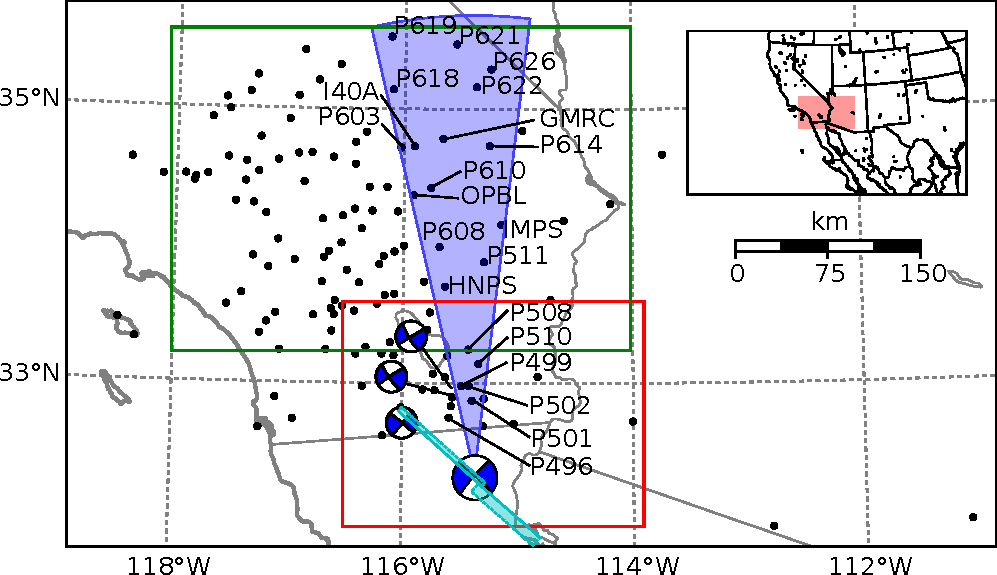
\includegraphics[scale=0.9]{Figures/context_map}
\centering 
\caption{}
\label{fig:ContextMap}
\end{figure}

\begin{figure}
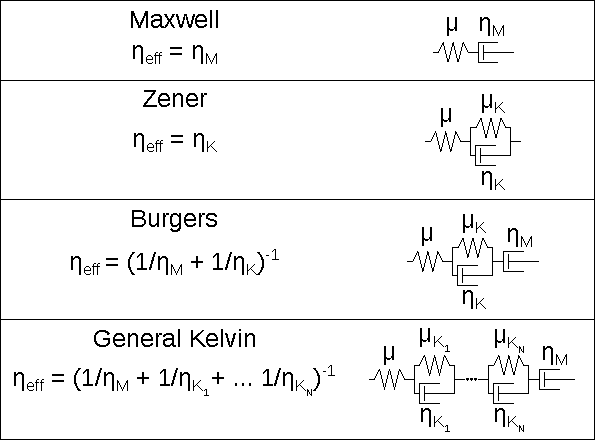
\includegraphics[scale=0.9]{Figures/rheology}
\centering 
\caption{}
\label{fig:Rheology}
\end{figure}

\begin{figure}
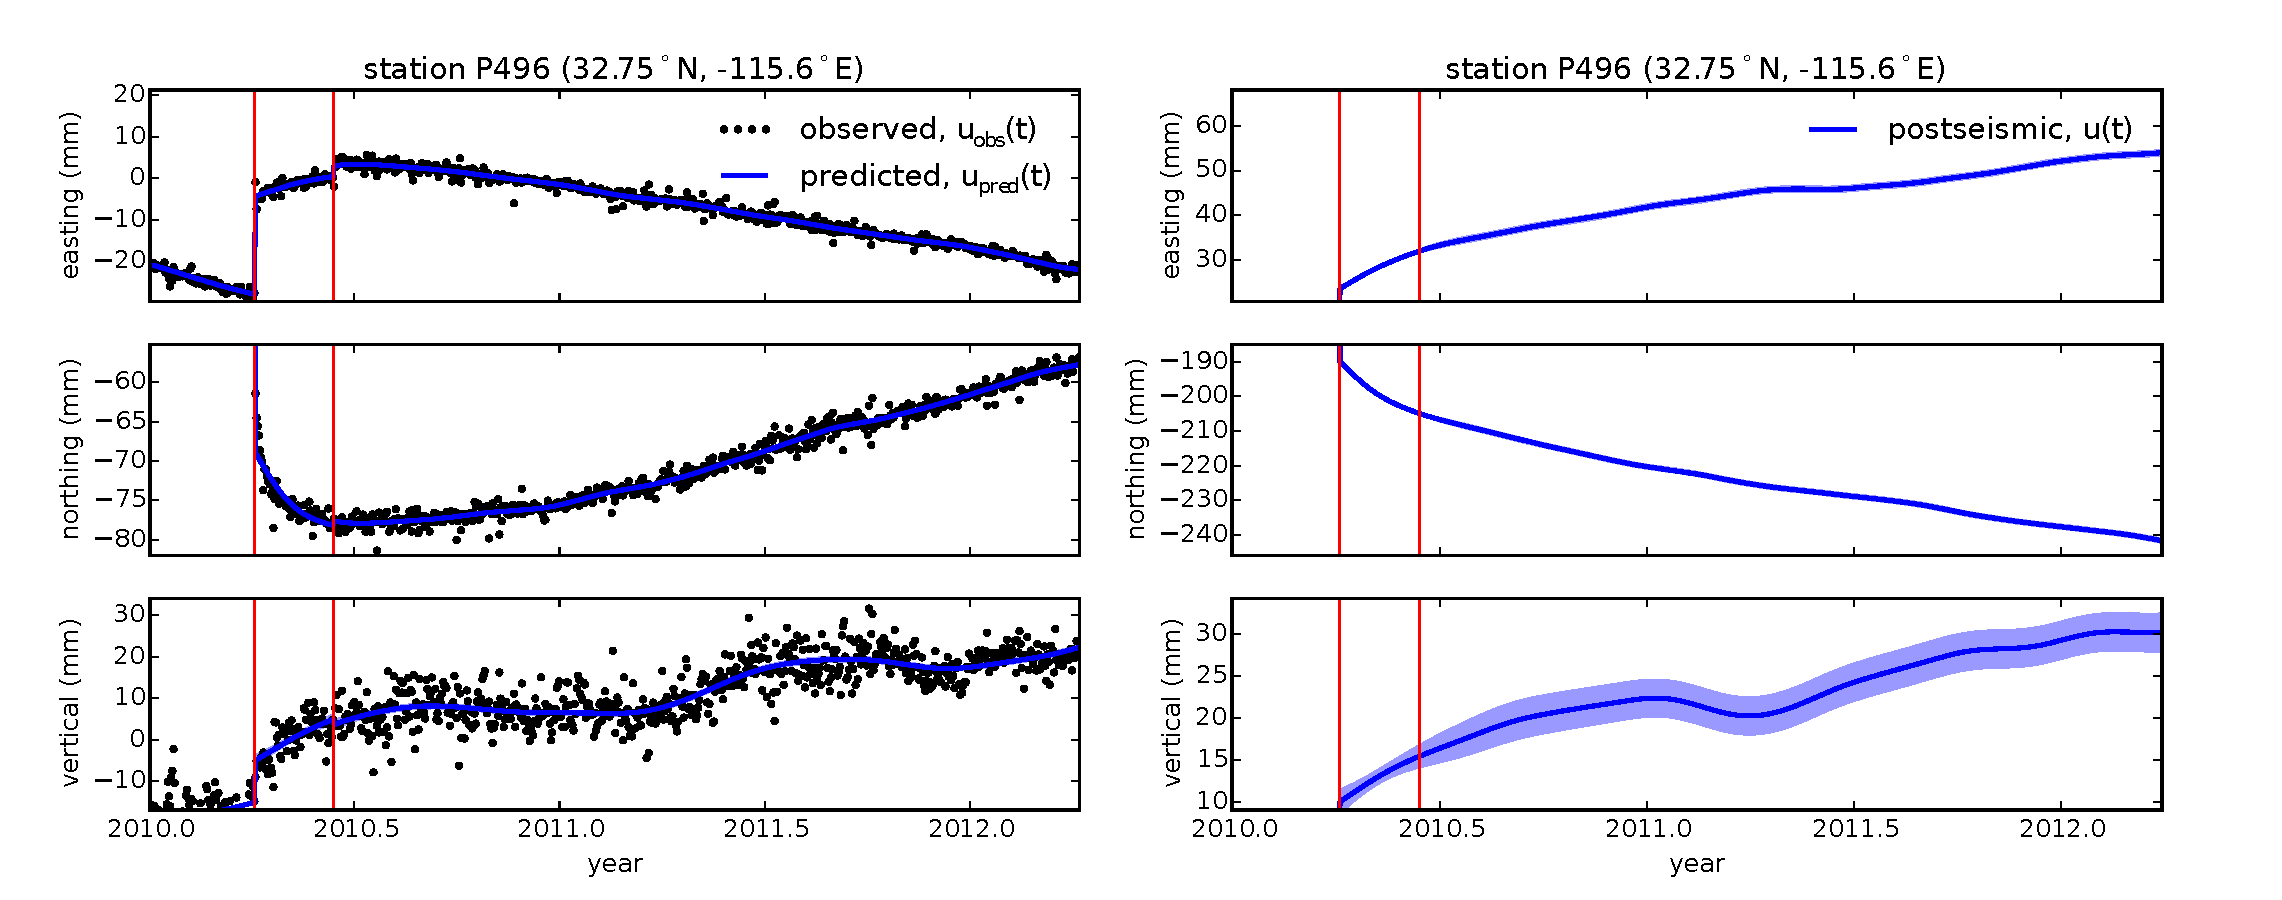
\includegraphics[scale=0.45]{Figures/filterP496}
\centering
\caption{}
\label{fig:P496}
\end{figure}

\begin{figure}
\includegraphics[scale=0.45]{Figures/filterP619}
\centering
\caption{} 
\label{fig:P619}
\end{figure}

\begin{figure}
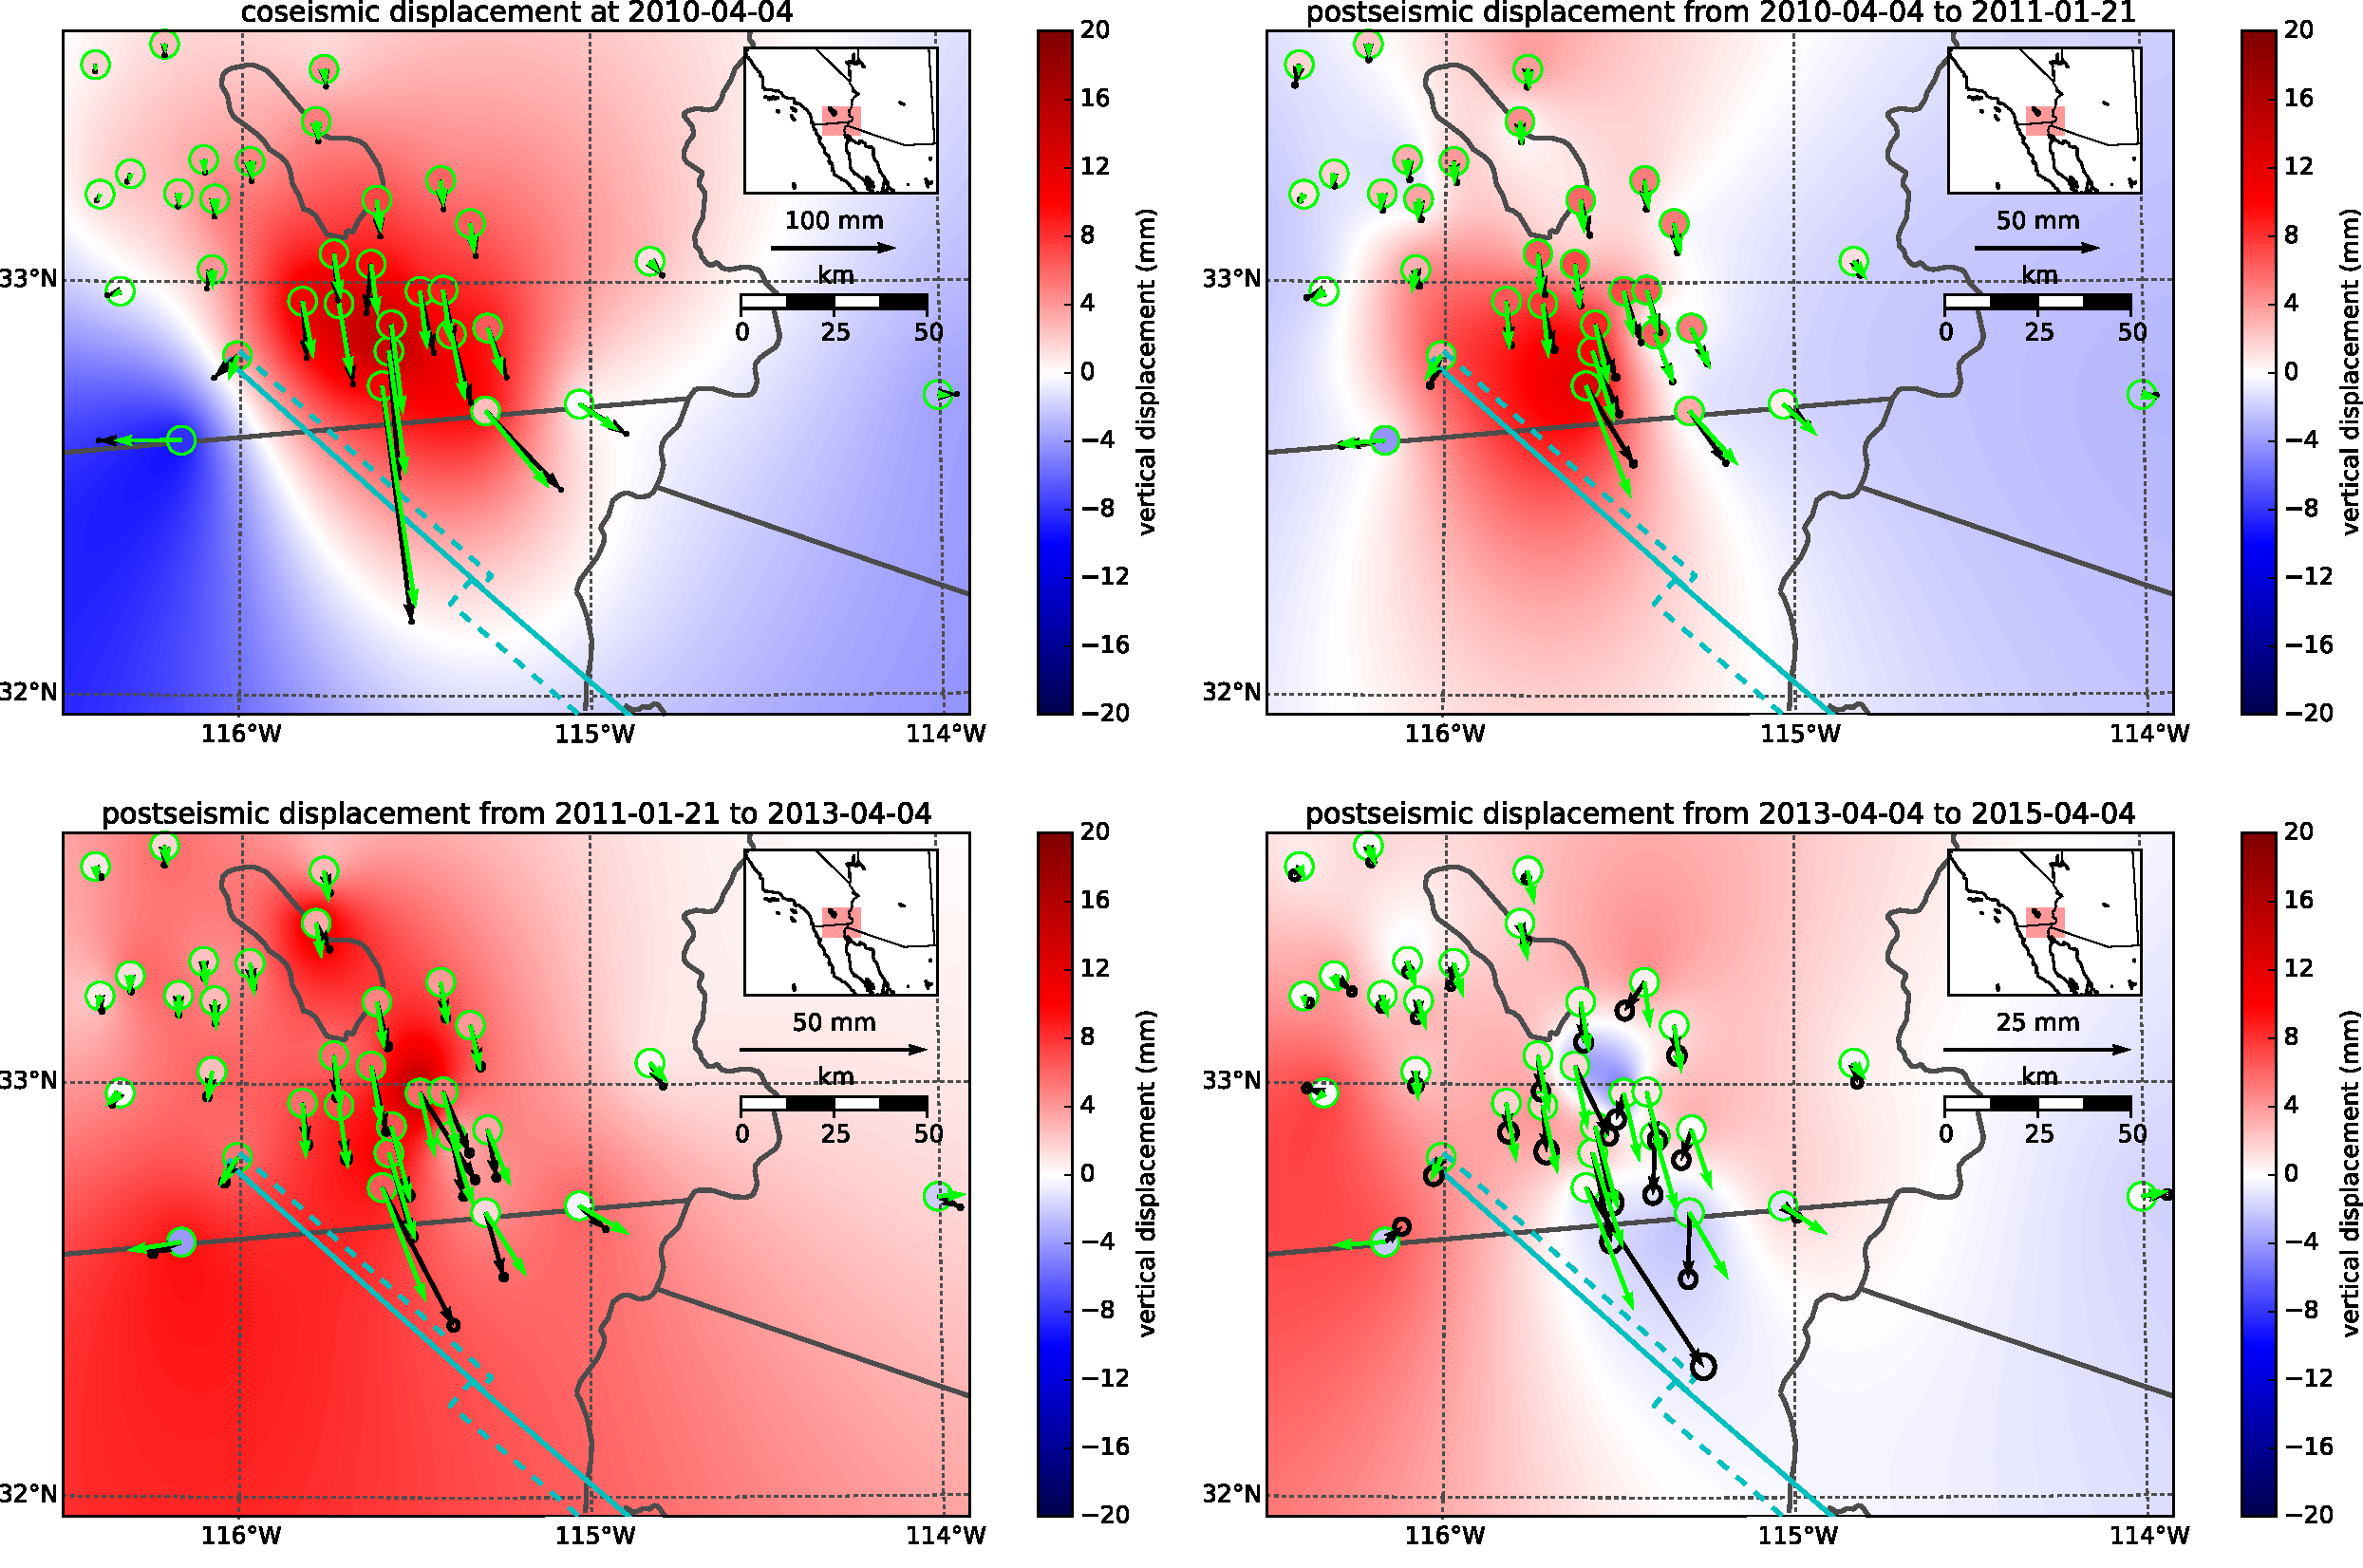
\includegraphics[scale=0.4]{Figures/nearfield}
\centering 
\caption{}
\label{fig:NearField}
\end{figure}

\begin{figure}
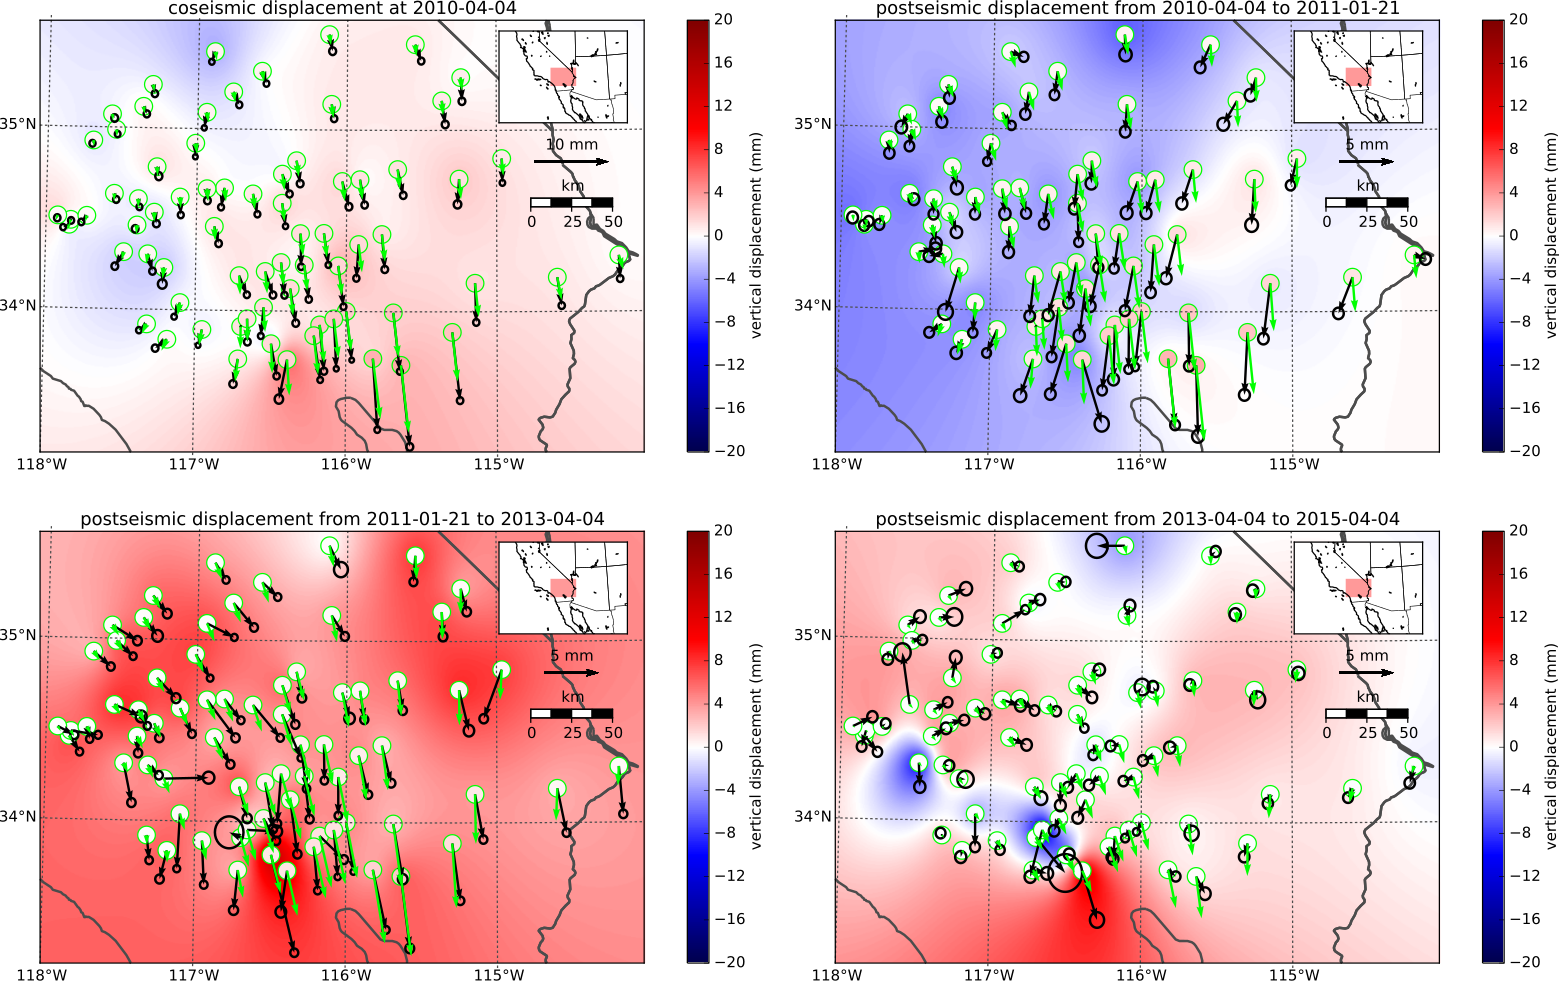
\includegraphics[scale=0.4]{Figures/farfield}
\centering 
\caption{}
\label{fig:FarField}
\end{figure}

\begin{figure}
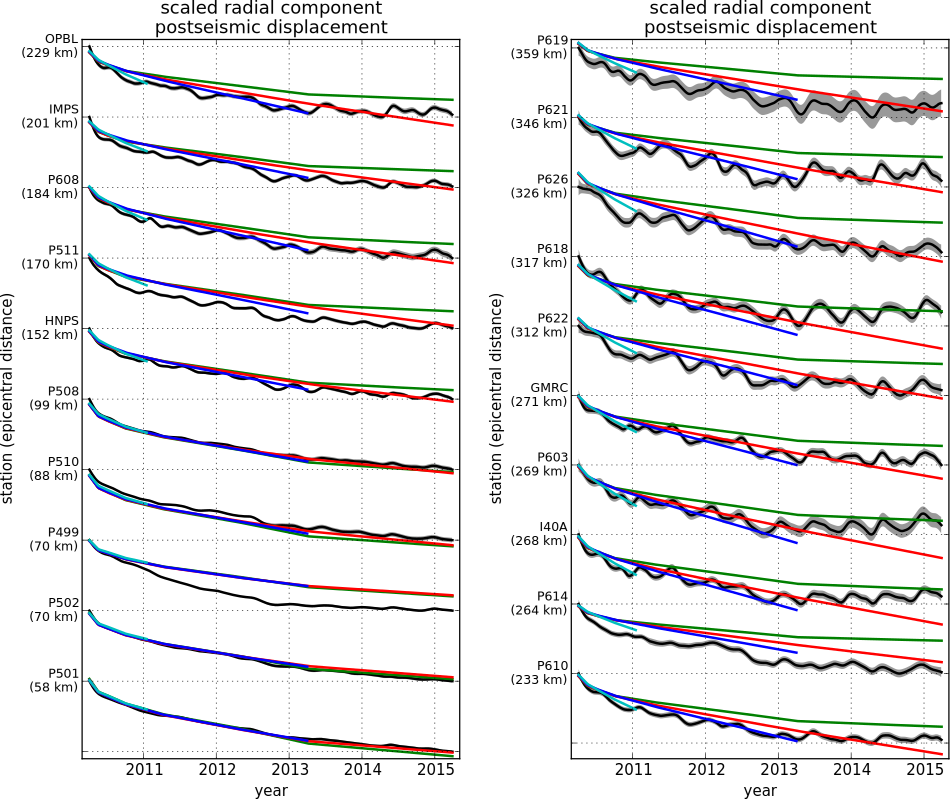
\includegraphics[scale=0.6]{Figures/recordsection1}
\centering 
\caption{record section}
\label{fig:RecordSection1}
\end{figure}

\begin{figure}
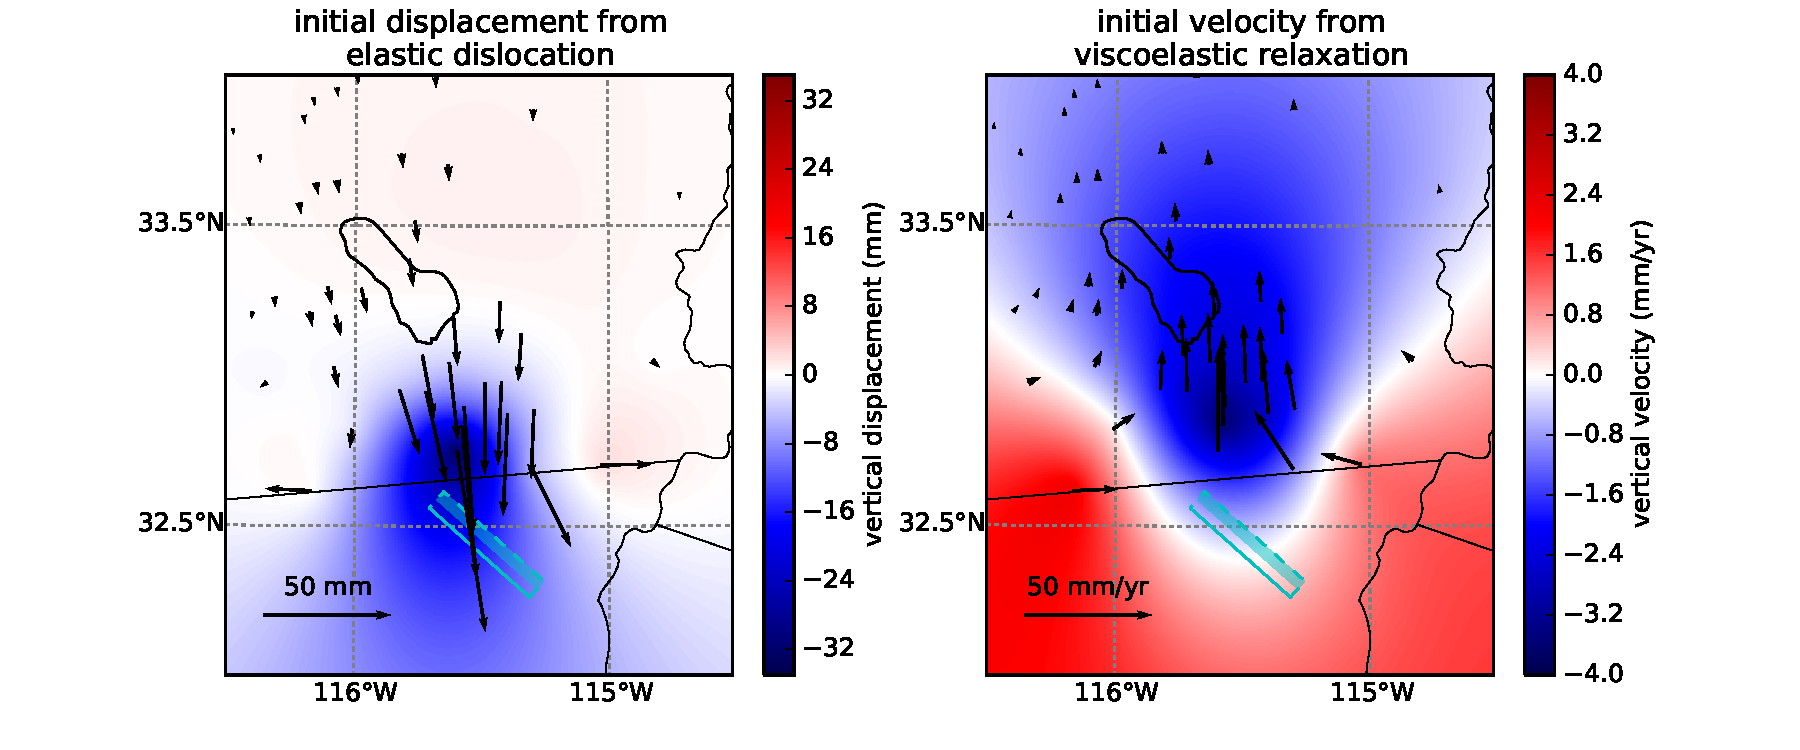
\includegraphics[scale=0.6]{Figures/lower_crust}
\centering 
\caption{afterslip and viscoelastic relaxation in lower crust}
\label{fig:LowerCrust}
\end{figure}

\begin{figure}
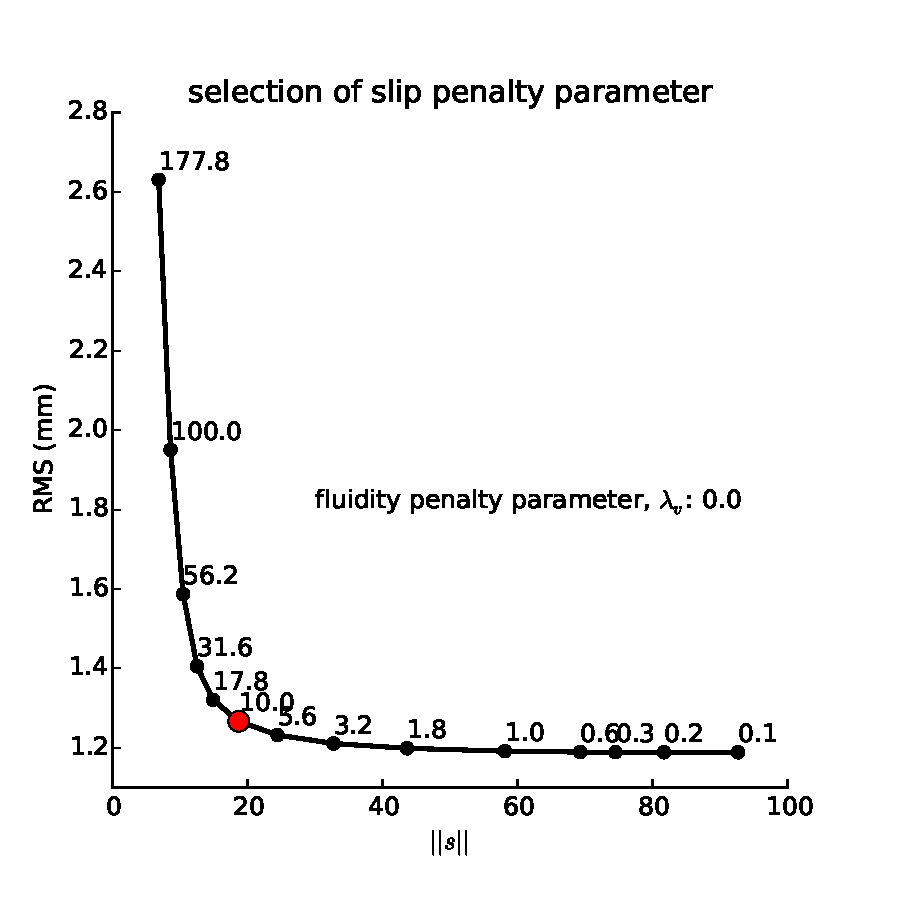
\includegraphics[scale=1.0]{Figures/slip_lcurve}
\centering 
\caption{near field record section}
\label{fig:SlipLCurve}
\end{figure}

\begin{figure}
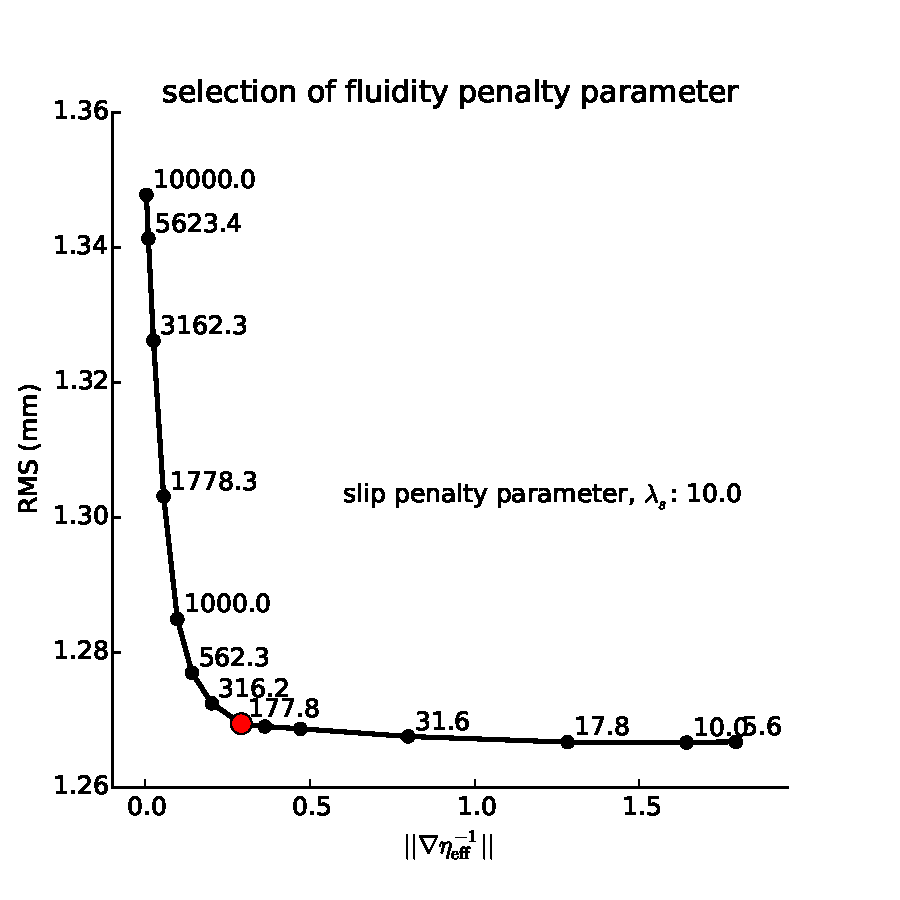
\includegraphics[scale=1.0]{Figures/fluidity_lcurve}
\centering 
\caption{far field record section}
\label{fig:FluidityLCurve}
\end{figure} 

\begin{figure}
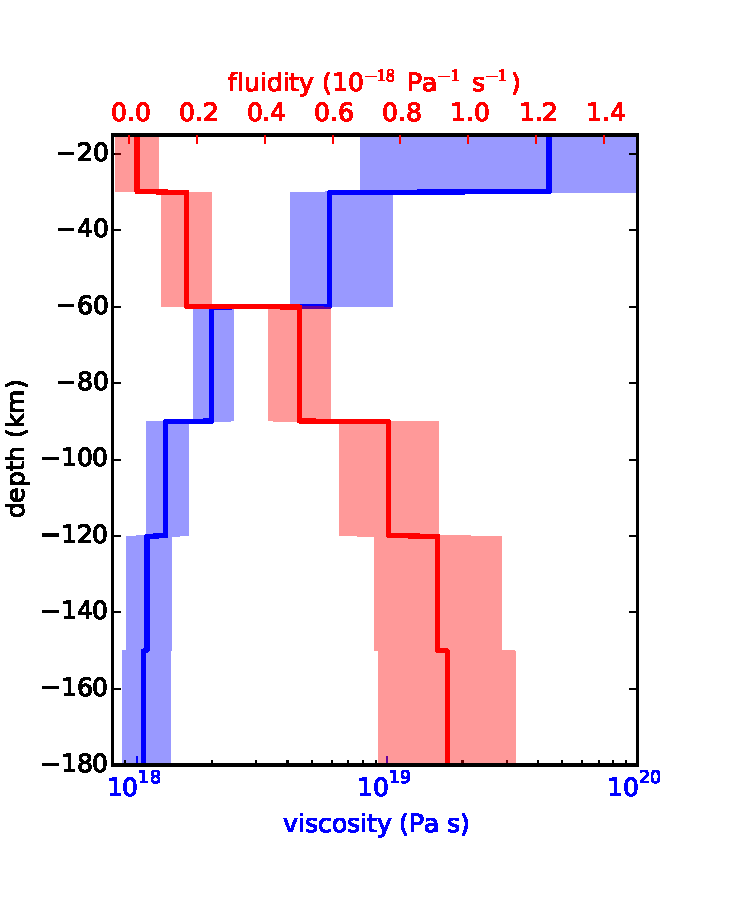
\includegraphics[scale=1.0]{Figures/effective_viscosity}
\centering 
\caption{effective viscosity}
\label{fig:EffectiveViscosity}
\end{figure} 

\begin{figure}
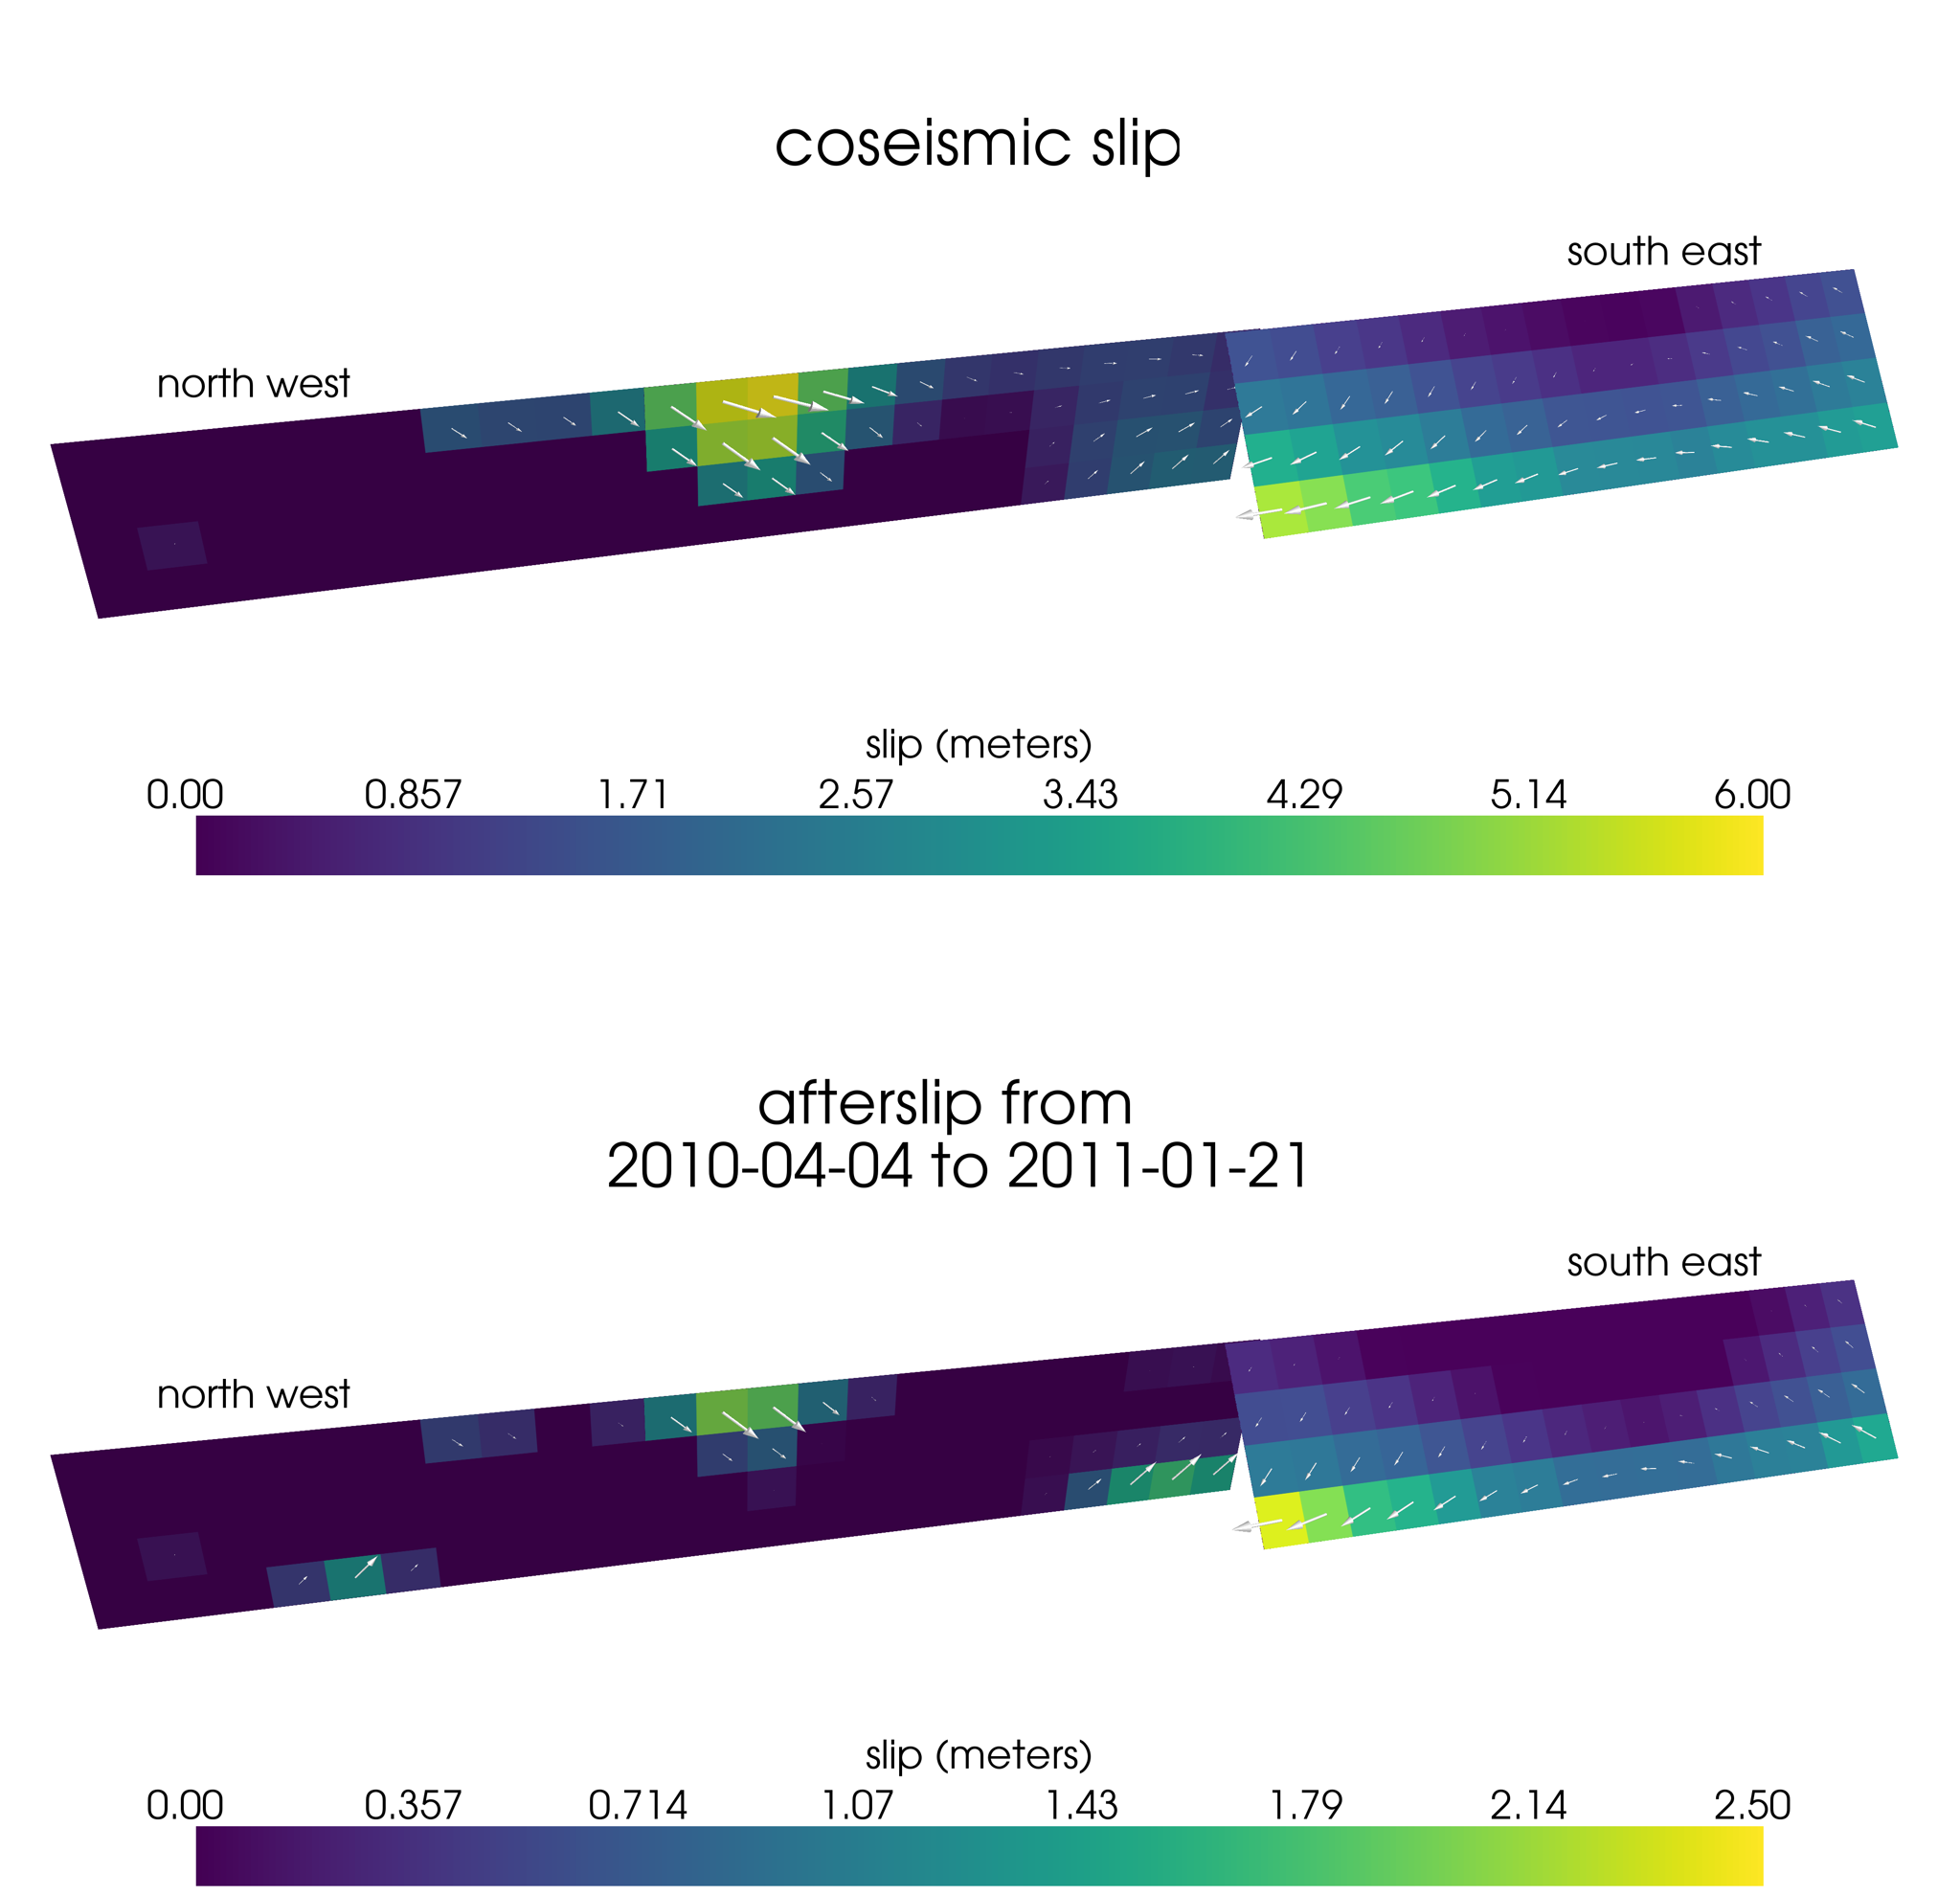
\includegraphics[scale=0.09]{Figures/initialslip}
\caption{}
\label{fig:InitialSlip}
\end{figure} 

\begin{figure}
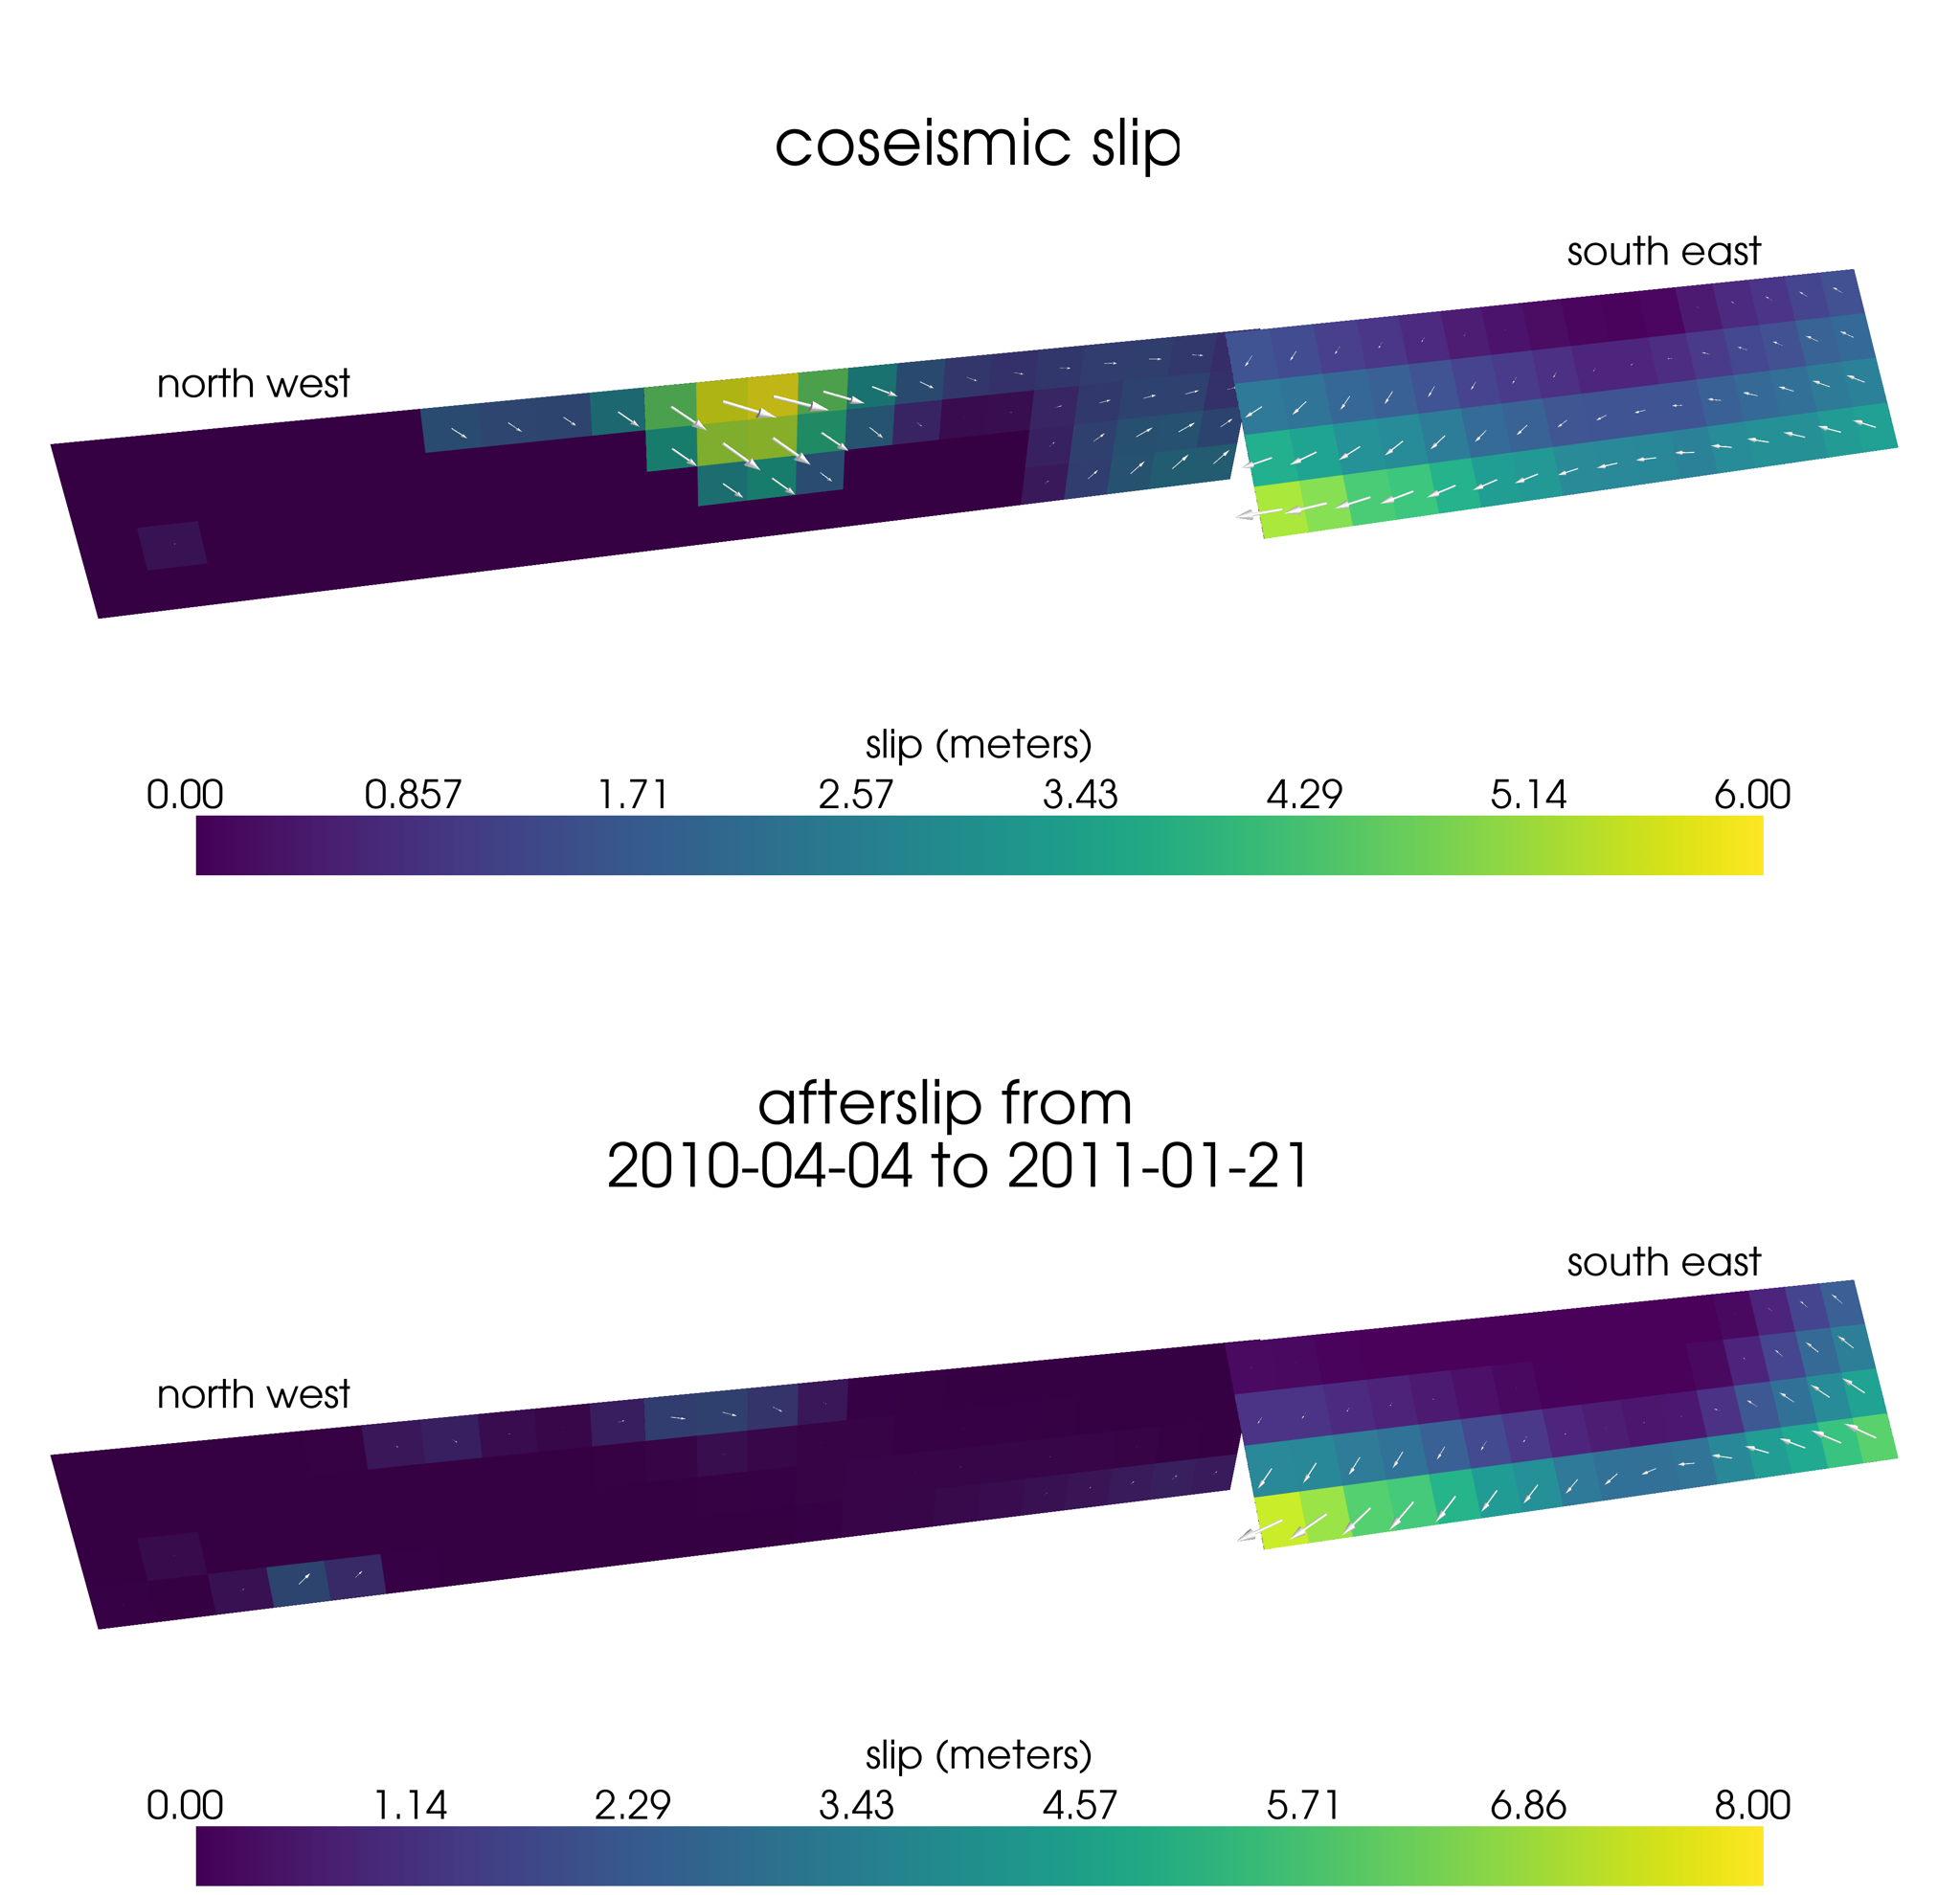
\includegraphics[scale=0.09]{Figures/elasticslip}
\caption{}
\label{fig:InitialSlip}
\end{figure} 


\begin{figure}
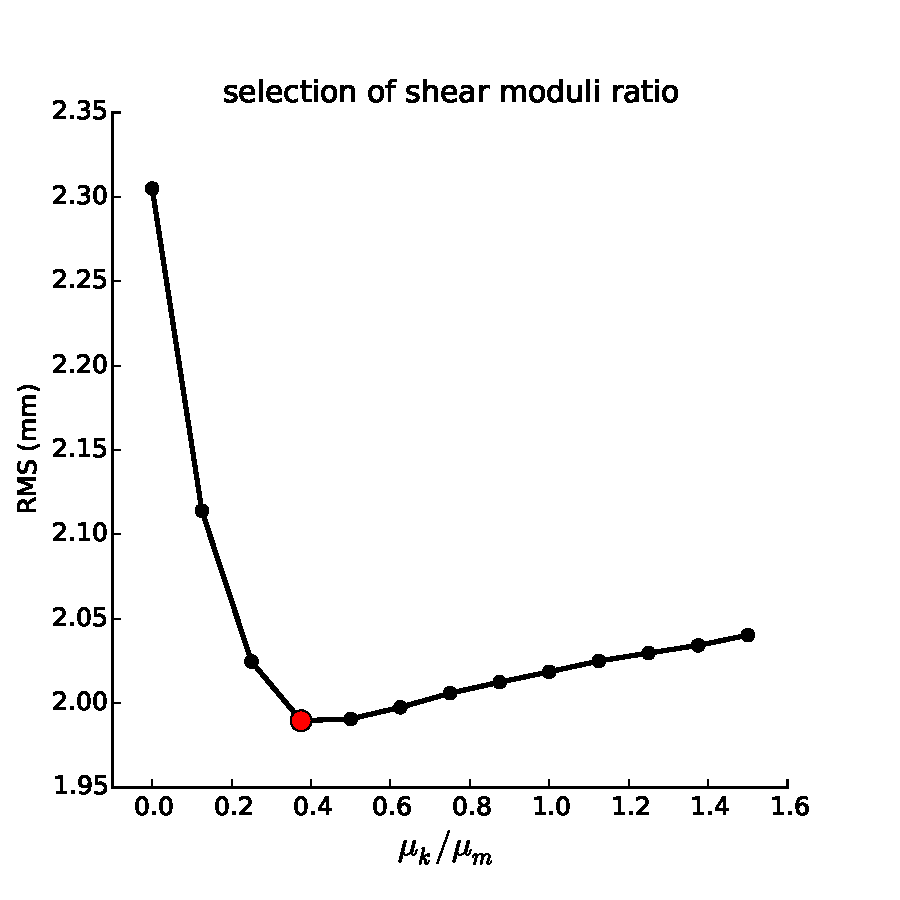
\includegraphics[scale=1.0]{Figures/shear_ratio}
\centering 
\caption{misfit with different shear modulus ratios}
\label{fig:ShearModulusRatio}
\end{figure} 

\begin{figure}
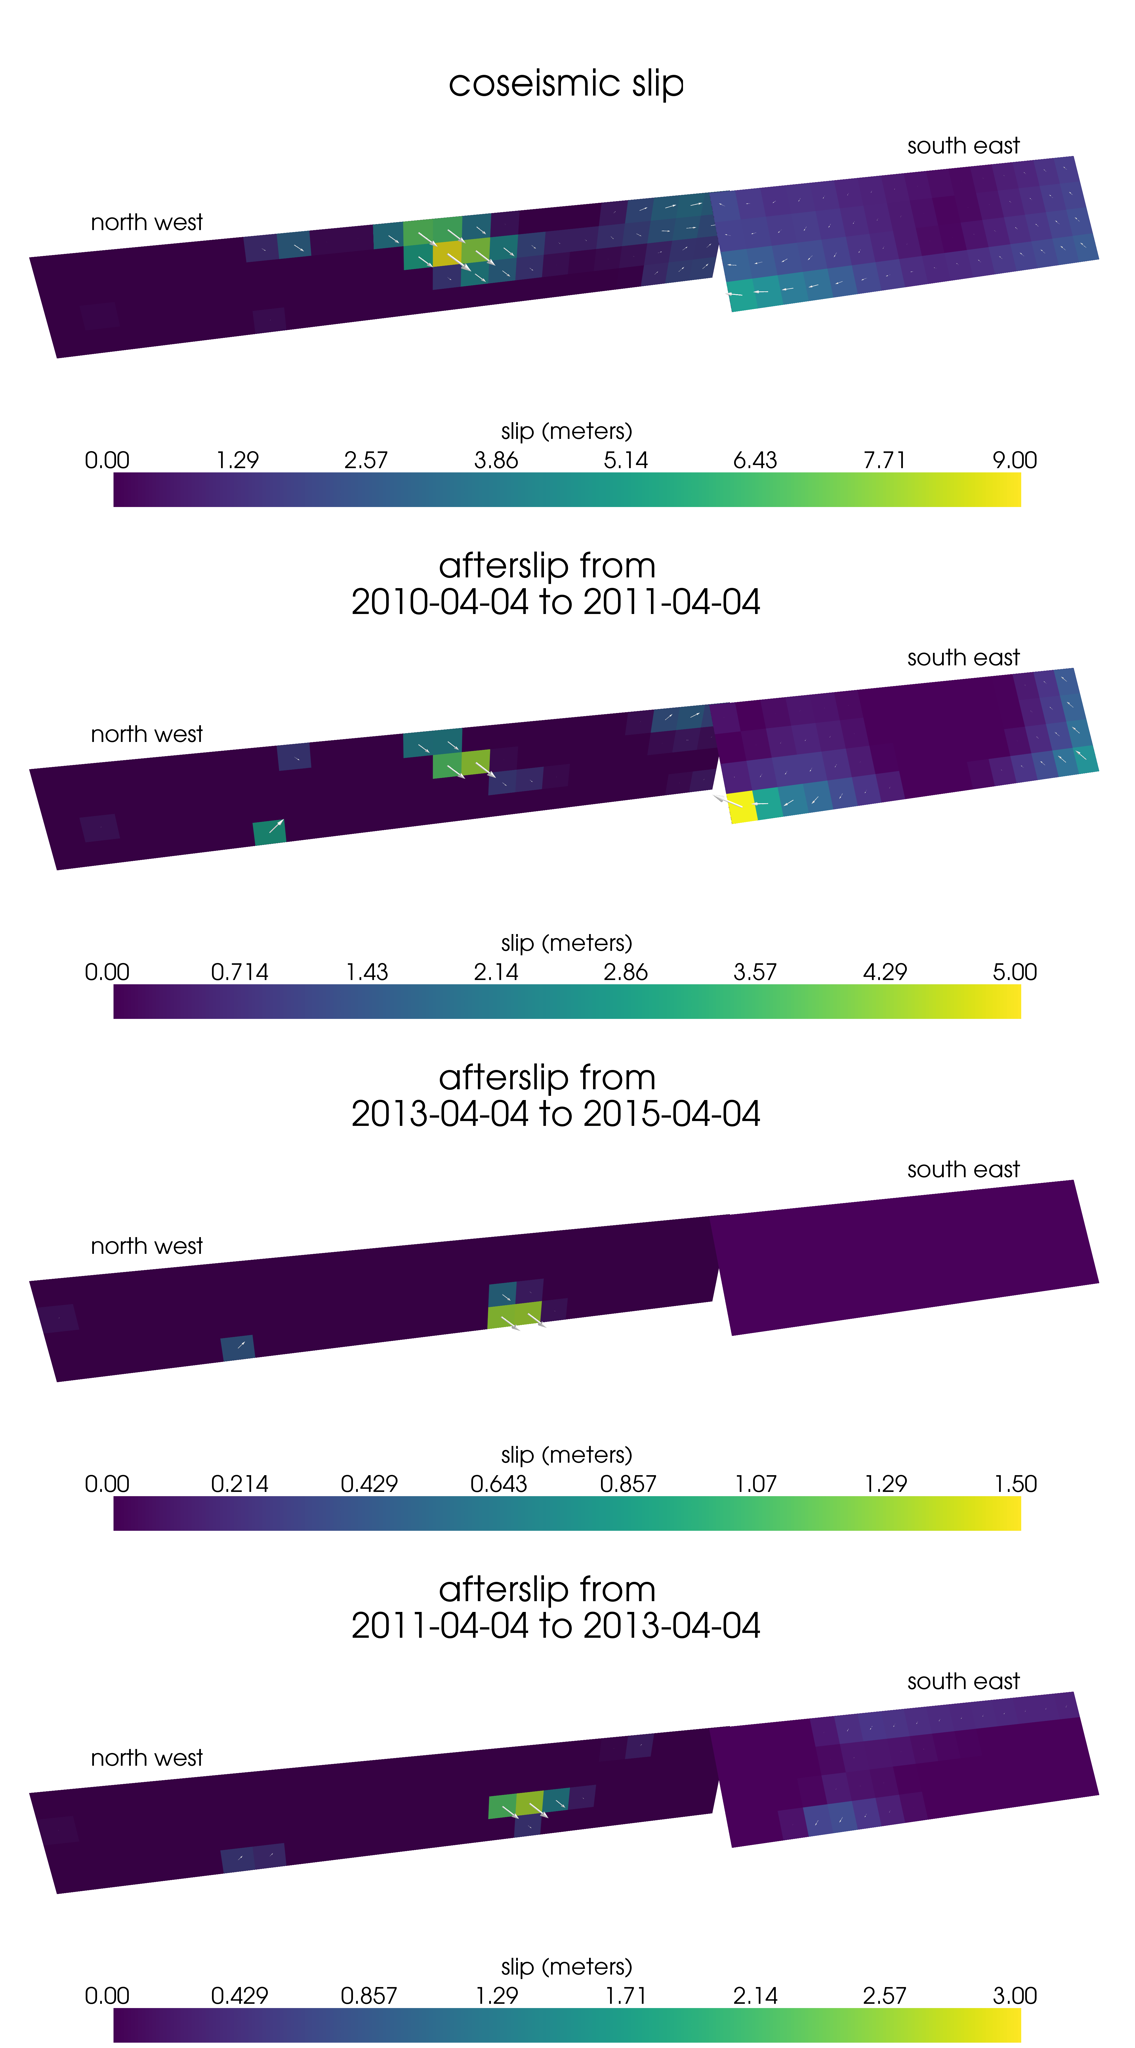
\includegraphics[scale=0.09]{Figures/finalslip}
\centering 
\caption{}
\label{fig:FinalSlip}
\end{figure} 


\begin{figure}
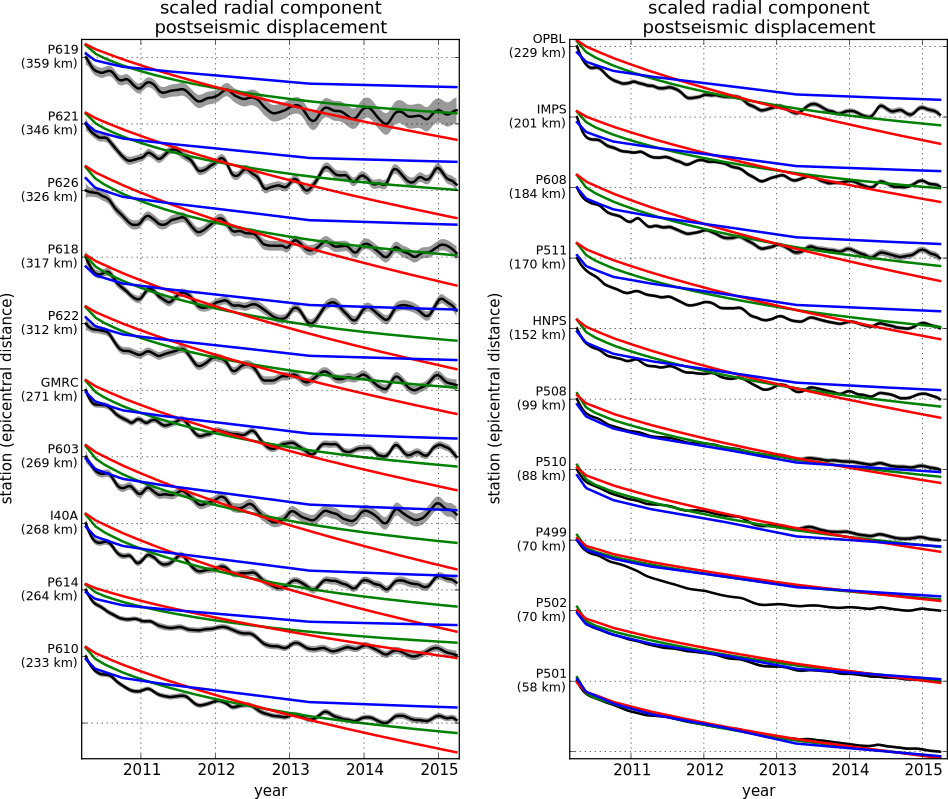
\includegraphics[scale=0.6]{Figures/recordsection2}
\centering 
\caption{}
\label{fig:RecordSection2}
\end{figure} 


\end{document}

